\documentclass[11pt, final]{westhesis}
\usepackage{graphicx} % Required for inserting images
\usepackage{tikz}
\usepackage[bookmarksdepth=3, colorlinks, allcolors=blue]{hyperref}
\usepackage{fancyvrb}

\usepackage{amsmath,amsfonts}
\usepackage{amssymb}
\usepackage{enumitem}
\setlist{nosep}

\usepackage{url}
\usepackage{natbib}

\newtheorem{theorem}{Theorem}
\newtheorem*{theorem*}{Theorem}
\newtheorem{definition}{Definition}
\newtheorem{definition*}{Definition*}
\newtheorem{lemma}{Lemma}
\newtheorem*{lemma*}{Lemma}
\title{On the Complexity of $k$-best and $2nd$-best Optimization Problems}
\author{Iain McLaren}
\date{April 2024}
\submitdate{April 2024}
\department{Mathematics and Computer Science}
\advisor{Daniel Krizanc}
\departmentname{Math and Computer Science}
\makeindex

\newcommand*{\exobt}{{Ex-2nd-Opt-Best}}
	
\newcommand*{\inobt}{{In-2nd-Opt-Best}}
\newcommand*{\exbt}{{Ex-2nd-Best}}
\newcommand*{\inbt}{{In-2nd-Best}}
\newcommand*{\exobk}{{Ex-$k$th-Opt-Best}}
\newcommand*{\inobk}{{In-$k$th-Opt-Best}}
\newcommand*{\exbk}{{Ex-$k$th-Best}}
\newcommand*{\inbk}{{In-$k$th-Best}}

\newcommand*{\pp}{{P}}
\newcommand*{\np}{{NP}}
\newcommand*{\nph}[1]{{NP\text{-Hard{#1}}}}
\newcommand*{\npc}{{NP\text{-Complete}}}

\newcommand*{\tpp}{{\text{Turing}-P}}
\newcommand*{\tnp}{{Turing-NP}}
\newcommand*{\tnph}[1]{{Turing-NP-Hard{#1}}}
\newcommand*{\tnpc}{{Turing-NP-Complete}}


\newcommand*{\exobht}{{Ex-2nd-Opt-Best-Hard}}
\newcommand*{\inobht}{{In-2nd-Opt-Best-Hard}}
\newcommand*{\exbht}{{Ex-2nd-Best-Hard}}
\newcommand*{\inbht}{{In-2nd-Best-Hard}}

\newcommand*{\exobhk}{{Ex-$k$th-Opt-Best-Hard}}
\newcommand*{\inobhk}{{In-$k$th-Opt-Best-Hard}}
\newcommand*{\exbhk}{{Ex-$k$th-Best-Hard}}
\newcommand*{\inbhk}{{In-$k$th-Best-Hard}}

\newcommand*{\exob}{\exobt}
\newcommand*{\inob}{\inobt}
\newcommand*{\exb}{\exbt}
\newcommand*{\inb}{\inbt}
\newcommand*{\exobh}{\exobht}
\newcommand*{\inobh}{\inobht}
\newcommand*{\exbh}{\exbht}
\newcommand*{\inbh}{\inbht}


\begin{document}

\begin{abstract}
Research in $k$-best computation and enumeration has historically been limited almost exclusively to problems with known polynomial-time solutions. We expand the field of study by focusing on the computational complexity of finding the second-best and $k$-best solutions to $\nph{}$ combinatorial optimization problems. We introduce several new problem classes and analyze their complexity for a wide range of well-known combinitorial optimization problems. Our results show that, in most cases, finding the second-best or $k$-best solution is itself an $NP$-hard task, even when the optimal solution is provided as part of the input. We also develop a general framework for proving the hardness of these problems in the future as well as identifying  notable exceptions to the general rule. This thesis lays the foundation for future research on the complexity of $k$-best optimization problems and highlights the potential for further investigations into $k$ and second-best $\nph{}$ problems.
\end{abstract}


\begin{acknowledgements}
    At times, when working on highly theoretical research such as this thesis, it is easy to feel dissuaded or stuck. That makes it even more important to have a network of support around you that encourages you to push on through the hardest parts. I am incredibly excited to have had the opportunity to study in this field and write this thesis, and I am so deeply grateful to everyone who has helped me along the way. I could not be happier with how it has turned out, and I have my own support network to thank for that.

    First, I would like to express my deepest gratitude towards my advisor, Professor Danny Krizanc. Throughout my semesters of research, he has been a constant source of advice and support. I would never have been able to write this thesis without his wealth of knowledge and insight.
    
    I would also like to thank my reading committee, Victoria Manfredi and Sonia Roberts, for taking the time out of their schedules to consider my thesis for the honors program. It really is appreciated.

    To my incredible family, you are the reason I could write this thesis in the first place. My parents, Susan and Campbell McLaren, have supported me in every way possible as I navigated college life. My siblings, Campbell and Jacqueline McLaren, have always been there for me, encouraging me every step of the way.

    Finally, I am so thankful to all of my friends at Wesleyan and beyond. Thank you for putting up with me when I was taking as many credits as I could fit into a semester to finish my three majors.

    
    
\end{acknowledgements}



\frontmatter
\maketitle
\makededication
\makeack
\makeabstract
\tableofcontents

\mainmatter

\chapter{Introduction}
Arguably the most famous open problem in computer science is the question of whether or not \textit{\textbf{P=NP}}. At a high level, it is the question of whether all problems for which an algorithm can \textit{quickly} check whether a specific answer is correct must also permit a fast algorithm that finds a correct answer from scratch. If anyone is able to solve the problem, they would be given a \$1 million cash prize from the Clay Mathematics Institute, as well as be inducted into Computer Science history. While we will not attempt to solve this infamous problem, we will continue to build on the shoulders of giants and add to the existing understanding of these complexity classes. In particular, we will focus on $k$-best optimization problems and expand the collective knowledge of these problems by specifically focusing on existing \nph{} problems. Before we can do that, though, we must define some terminology.
\section{Preliminaries}
\subsection{P and NP}
Let us first define our problem space. Formally, \textit{\textbf{\pp{}}} is the set of problems that a deterministic Turing Machine can solve in an amount of processes that is polynomial in the size of the input. The word ``deterministic" is key in this context, as it means the machine must only be able to perform a single action at once, decided entirely by its state and programming. On the other hand, if a problem is solvable by a non-deterministic Turing Machine in polynomial time on the size of the input, then it is considered to be in \textit{\textbf{\np{}}}. A non-deterministic Turing Machine is capable of performing multiple actions at once. In modern computing, it can be thought of as a perfectly parallel processor, but the important thing to note is that a non-deterministic Turing Machine, when choosing between possible paths down its state tree, will always choose the path that eventually leads to the optimal solution -- at least when one exists. While this non-deterministic machine is the original idea that creates the class of $\np{}$ problems, it is often easier to consider the equivalent formulation of a verifier. A problem is $\np{}$ if any algorithm exists that can, in polynomial time on the size of the input, confirm that a provided feasible solution is an actual solution to a problem. Thus, intuitively, non-deterministic machines seem explicitly more capable than polynomial machines. They can ``guess" the answer to a question, and be sure that they are correct. This leads many researchers to the hypothesis that $\pp{} \subsetneq \np{}$, or that every $\pp{}$ problem must be solvable by a non-deterministic machine but that the reverse is not true. However, this belief has yet to be rigorously proven, and many computer scientists are still actively searching for polynomial time algorithms that break the mold and could prove that, in fact, $\pp{} = \np{}$. 
\subsection{NP-Hardness}
In the world of $\np{}$, there are two especially interesting classes of problems. Since non-deterministic polynomial machines are certainly not in any way weaker than their deterministic counterparts, it is obvious that any problem in $\pp{}$ must also be in $\np{}$, i.e. $\pp \subseteq \np$. This leads to the natural distinction of problems that are in $\np{}$ and yet likely not in \pp. One way to define problems that meet this description is with the \textit{\textbf{\nph{}}} problems. This is a set of computable problems that are ``at least as hard" as all other problems in $\np{}$. That means that if we find a way to solve any of these problems in polynomial time with a deterministic machine, we can solve every problem in $\np{}$ in polynomial time, and thus $\pp{} = \np{}$. This class of $\nph{}$ problems is constantly growing as more and more researchers find new tasks that fall under the category. The proof that a problem is $\nph{}$ is not necessarily complicated. If we want to prove that problem $B$ is $\nph{}$, we would need to prove that there is a polynomial time deterministic algorithm that can convert the input of an existing $\nph{}$ problem, $A$, into that of the examined problem $B$. If we can then show that answer of the produced input on $B$ is the same as answer to the original input for problem $A$, we have shown that $B$ is an $\nph{}$ problem. This ``conversion" algorithm is referred to as a many-one reduction, or a Karp reduction. An alternative reduction, called a Turing reduction, is also occasionally used in complexity analysis. Unlike Karp reductions, Turing reductions permit the repeated use of an algorithm that solves $B$ in our attempt to solve $A$. In other words, Turing reductions can be thought of as programs that can use a subroutine -- often called an oracle -- that solves our examined problem $B$ in order to solve an existing $\nph{}$ problem $A$ in polynomial time. This makes Turing reductions a superset of Karp reductions; every Karp reduction is a Turing reduction but not necessarily the other way around. This does however make Turing reductions more powerful which in turn makes them less distinguishing, and thus Karp reductions have become the gold standard in complexity analysis. Where possible, and unless otherwise noted, this thesis will use Karp reductions. 
\subsection{NP-Completeness}
In the above section, we mentioned that $\nph{}$ problems are at least as hard as all problems in $\np{}$. As this statement implies, there are problems that are even more difficult than \np{}. Even non-deterministic Turing Machines can't solve these types of problems efficiently. While this thesis will not deal extensively with these problems, they do necessitate a final distinction, the \textit{\textbf{\npc{}}} class of problems. These are simply problems that are both $\nph{}$ and $\np{}$, that is they can be solved in polynomial time by a non-deterministic machine, but they also can be used to quickly solve all other problems in \np{}, thus likely seperating them from all of the problems in $\pp{}$, so long as $\pp{} \neq \np{}$.
\subsection{Decision and Optimization Problems}
We have so far defined the concept of a computational ``problem" somewhat loosely, so let us deal with this term more rigorously. We will deal with two particular types of problems. The first are \textbf{decision problems}. Given a general language $L$ that contains all input strings valid for our problem, the language of a decision problem takes the following form: $\{{} I \in L : \mathcal{P}(I)\}$ where $\mathcal{P}$ is a predicate that is either true or false on all input strings in $L$. In other words, it is the set of all strings in $L$ that are true under the predicate of the problem. Intuitively, decision problems can be thought of as problems that are solved by an algorithm that accepts inputs of a certain type and returns exclusively true or false. All $\npc{}$ problems are of this form. We can greatly expand the number of interesting problems if we consider \textbf{optimization problems}, as these are some of the most common to come about in the real world. Consider instead a problem in which we have a set of possible solutions $S$, and we are given a cost function $C : S \rightarrow{} \mathbb{R}$. An optimization problem is a problem in which the machine must determine the solution $s \in S$ such that $C(s)$ is either minimized or maximized. Any maximization or minimization optimization problem can be easily reduced into the other with a simple sign flip of the cost function, so we will henceforth simply refer to the minimization of the cost function when considering general optimization problems. Specific problem instances for which maximization is more natural will remain unchanged, so this note is only important when discussing the problems in a general sense. While optimization problems cannot themselves be considered $\npc{}$, we can often craft a decision problem from these. The most common way of doing this is to use the same formulation as the optimization problem, but add an parameter $t$ into the input, so that instead of asking the algorithm to optimize, we ask whether or not there is a solution with cost lower than $t$. Unless otherwise stated, any time we refer to the ``decision form" of what is otherwise an optimization problem, we are referring to this formulation. In the world of optimization problems, we can even further specify \textbf{combinitorial optimization problems}. These are optimization problems in which the set of feasible solutions, $S$, is discrete. Combinitorial optimization problems will be the primary focus for this thesis, as it is only for these types of problems that there is a natural definition of $k$-best solutions.
\subsection{$k$-Best Combinitorial Optimization Problems}
Now that we have most of the necessary terminology available, we can look more closely at the subject of this thesis. While for some problems, we really only do care about the one-and-only optimal solution, for many real world situations this is not the case. This is where $k$-best algorithms come into play. Instead of taking in the standard input for an optimization problem and searching for the optimal solution, a $k$-best algorithm will also have an enumeration value, $k$, and will output the top $k$ optimal solutions according to the cost function. At first, it may seem useless to do so much additional work just to find worse solutions, but there are plenty of instances where it is helpful. Recently in my own life, I was planning a trip through Europe with some of my friends for after graduation. It involved possible routes between dozens of different cities. I didn't want to just find the single cheapest or shortest route between all these different locations, I also wanted to compare that ``best" route with other good routes to see how much better it was, and whether there were other factors I could consider that might make the ``good, but suboptimal" solutions even better than the ``optimal" solution. This is just one application of a $k$-best combinitorial optimization problem, and is functionally equivalent to the $k$-best travelling salesman problem discussed later in this thesis.

Beyond personal experience, in many real-world cases the optimal solution can be unstable or fragile; small changes to the initial conditions could drastically alter the optimality of a solution. Having a collection of very good options instead of one single solution could improve the robustness of the algorithm, preventing small changes from creating large-scale issues \cite{kurtz2023approximation, kalyanmoy2006in}. Some areas of study that this may be particularly useful are in machine learning, internet network routing, and transportation routing, where it is not uncommon for small changes in the system can lead to sweeping changes in the outcome if not properly accounted for. 

In the end, most computer models can be considered an approximation of what is happening in the real world, thus making it important to compare the calculated optimal solution against its rivals. 
\section{Related Work}
The study of second-best and $k$-best solutions is closely tied to the overarching field of computational complexity theory. The seminal works of Cook \cite{cook1971complexity}, Levin \cite{levin1973universal}, and Karp \cite{karp1972reducibility} established the foundations of reducibility, NP-hardness, and NP-completeness. In order to understand the hardness of $k$-best problems, we must first have a detailed understanding of the basis of the field and the various existing complexity classes. Garey and Johnson's book \cite{garey1979computers} serves as a comprehensive guide to the theory of NP-completeness and many of the known problems that have no efficient solutions, assuming that indeed $P \neq NP$. Finally, the famous, or perhaps infamous, ``Introduction to Algorithms" by Cormen et al. \cite{CLRS} textbook is a must-have for any researcher in algorithms and complexity theory.

Delving specifically into our focus, the problems of finding the $2nd$-best or $k$-best solutions to combinatorial optimization problems date back decades. Four years before Richard Karp produced the previously mentioned paper defining the class of NP-Complete problems, Murty published an establishing work in the field of $k$-best problems, showing that the assignment problem, a well-established problem in P, permits an efficient algorithm to enumerate the $k$-best solutions \cite{murty1968letter}. Three years later, in 1971, Yen is able to do the same for the shortest path problem, another problem with a known polynomial algorithm for finding the optimal solution. This algorithm is still highly useful to this day, as there are many applications in which it may be helpful to see a handful of the shortest paths through a graph, for instance when selecting a route on Google Maps that differs from the fastest route. Importantly, the time complexity of each of these algorithms is at least linear in $k$. Since $k$ is an integer, and binary encodings of integers grow exponentially in the size of the integer, the time complexity of these algorithms is technically also exponential in input size. This is often referred to as a pseudopolynomial time algorithm. It may be an interesting area of further study to constrain $k$ not just to the $2nd$-best, but to some sort of theoretical ``breaking point", where a problem no longer has a strongly polynomial time algorithm to find the $k$th-best solution.


One year after Yen's paper, in 1972, Lawler published one of the most important papers ever produced in the field \cite{lawler1972procedure}. In his work, he is able to expand the previous two approaches into a general approach for handling $k$-best enumeration problems. He describes a procedure to enumerate solutions in cost order by efficiently solving subproblems at each step.

Since then, numerous researchers have built upon these initial findings and developed more efficient algorithms for specific combinatorial optimization problems, as well as for problems in which Lawler's procedure isn't easily applicable. Gabow \cite{gabow1977finding} presented two algorithms for generating weighted spanning trees in order, which is equivalent to generating the $k$-best minimum spanning trees. His work introduced the practical concept of using a priority queue to efficiently generate solutions in increasing order of cost, a technique that has been widely adopted in later research, as well as expanded upon and improved for common constrained types of graphs \cite{katoh1981efficient, frederickson1993ambivalent}. Eppstein, a name which will come up all throughout this thesis for his constant efforts to expand recognition for $k$-best algorithms, \cite{eppstein1997finding} developed an algorithm for finding the $k$ shortest paths in a graph, improving upon Yen's earlier work in the area. His algorithm, which runs in $O(m + n + k)$ time when provided a shortest path tree and $O(m + nlog(n) + klog(k))$ otherwise, where $m$ is the number of edges and $n$ is the number of vertices in the graph, is particularly useful to assist with efficiently solving a variety of important dynamic programming problems.

The complexity of finding the second-best solution has also been studied for the minimum spanning tree problem. Katoh et al. \cite{doi:10.1137/0210017} presented an algorithm for finding the $k$ minimum spanning trees in an undirected graph. Their algorithm runs in $O(km + \min(n^2, m\log \log n))$ time and uses $O(k + m)$ space, where $n$ is the number of vertices and $m$ is the number of edges. This result shows that finding the second-best minimum spanning tree can be done efficiently for a fixed value of $k$.

However, the complexity changes when $k$ is part of the input. Ravi et al. \cite{ravi1996spanning} proved that finding the $k$th best minimum spanning tree is NP-hard for arbitrary values of $k$. This hardness result holds even for planar graphs and implies that, unless P=NP, there is no polynomial-time algorithm for finding the $k$-best minimum spanning trees when $k$ is not fixed.

These results highlight the interesting complexity landscape of finding second-best solutions, where the difficulty can depend on whether certain parameters, such as the value of $k$, are fixed or part of the input. The contrast between the polynomial-time algorithm for fixed $k$ and the NP-hardness for arbitrary $k$ in the case of minimum spanning trees provides a compelling example of this phenomenon.

The complexity of finding the second-best solution has also been studied for lesser-known problems. Camerini \cite{camerini1980complexity} generalized the existing work on weighted spanning tree enumeration into a paper on $k$-best spanning arborsecenses. Fukuda et al. was able to improve upon existing techniques to develop a much more efficient method to enumerate all perfect matchings in a bipartite graph \cite{fukuda1997finding}.

In addition to problem-specific algorithms, researchers have also developed general techniques for $k$-best enumeration. Fourty-eight years after Lawler publishes his generalized procedure to approach $k$-best problems, Eppstein \cite{eppstein2014k} provided an overview of $k$-best enumeration techniques and their applications, highlighting the importance of these methods in various practical fields especially in social, road, and internet networks. This survey was key in developing our own thoughts on the field and helped lead to the creation of this thesis. It is an excellent starting place for a new researcher in this field, and even deep into research I found myself returning to it as a useful reference. At the same time, it also shows how little research has previously gone into examining $k$-best $\nph{}$ problems, both in terms of developing better algorithms and in terms of establishing the complexity classes of such problems. The only reference in the survey to research into $k$-best problems where the original optimization problem is $\nph{}$ is referencing a technique commonly used in $\nph{}$ problems where we deal with ``parametrized complexity", where we can find a polynomial algorithm in some integer that defines the size of the input. Chen et al. use this technique to enumerate the top $k$ solutions to various $\nph{}$ problems \cite{chen2013par}, however their solutions require heavily constrained inputs and don't deal much in the actual hardness of the problem beyond the initial optimization problem.

Moving beyond Eppstein's work, Hamacher and Queyranne \cite{hamacher1982k} analyzed the existing Lawler approach and established their own procedure to enumerate the $k$-best solutions of various problems, which has been widely cited and extended in subsequent research \cite{yen2005finding, pascoal2013k}.

Other notable contributions to the field include the work of Papadimitriou and Steiglitz \cite{papadimitriou1982complexity} on the complexity of combinatorial optimization, which provides a detailed analysis of the algorithmic and complexity-theoretic aspects of optimization problems. Papadimitriou's work will be referenced multiple times in this thesis, particularly in the section on the Travelling Salesman Problem. There were several moments during the research process that we found a result only to read the following week that Papadimitriou has already proven something that was nearly the same more than 30 years prior. Valiant's work \cite{valiant1979complexity} on the complexity of enumeration and reliability problems has laid the foundation for the study of counting problems and their relationship to optimization.

In addition to the works mentioned above, there are many other research efforts that have been directed toward finding near-optimal solutions in combinatorial optimization, a similar but distinct problem. Powerful and complex techniques, both general and problem-specific, such as local search, approximation algorithms, and integer programming formulations, show the practicality of being able to rapidly find ``good" solutions that are not necessary optimal.

From this thought, some fields have been created and taken down entirely new avenues of research. One such field is matheuristics, a relatively niche study that I have only recently come across, in which a heuristic algorithm is combined with a solution improvement procedure using machine learning \cite{de2023mathematical}. A more well-known field, at least when it comes to the study of complexity theory, is the search for approximation algorithms and the study of NP-hard optimization using approximation algorithms. Particularly in this section, there have been a multitude of results pertaining to many of the problems covered later in this thesis, these include Max-Clique \cite{uriel2004approx}, Vertex-Cover \cite{karakostas2009better}, Independent Set \cite{chalermsook2023polynomial, berman1994approximating}, Set-Cover \cite{shi2019approx}, and Bin-Packing \cite{zhang2000linear}. Initially, we suspected there would be a correlation, if not a causation, between the difficulty of approximation for a problem and the difficulty of finding the second-best solution. While we weren't able to make conclusive headway in that area, we do still suspect some connection and will leave it for future work in the field to prove it one way or the other. In general, the sheer amount of work and results in related fields both illustrates the value of studying $k$-best problems and highlights the complexity and difficulty of working in the field. We had many questions to start the research, and were only able to answer some of them, while many others remain to be delved into by further research.  

\section{Established Approaches}
There are several approaches demonstrated by previous research in the field. Eppstein does an excellent job outlining them in \cite{eppstein2014k}, and we will summarize them here. 
\subsection{Optimal Substructures}
The optimal substructure approach leverages the principles of dynamic programming to solve $k$-best problems efficiently. In this method, the original problem is decomposed into a collection of subproblems, each of which is a smaller instance of the first problem. The key insight that permits the use of dynamic programming is that the optimal solutions to the original problem can be constructed by combining the optimal solutions of these subproblems in a specific manner, as described by a recurrence relation. We can use this fact to develop a similar technique to enumerate more than one good solution.

To apply this technique to $k$-best problems, instead of maintaining a single optimal solution for each subproblem, we store each of the $k$ best solutions. The recurrence relation is then adapted to express the $k$ best solutions of a subproblem in terms of the $k$ best solutions of smaller subproblems. Thus, we can use the dynamic programming algorithm to solve our own problem. At each step moving from smaller to larger subproblems, the recurrence relation is used to compute and store the $k$ best solutions for the current subproblem, based on the previously computed solutions of smaller subproblems.

This approach effectively extends the dynamic programming paradigm to allow the generation of multiple optimal solutions, enabling the efficient computation of $k$-best results for problems exhibiting optimal substructure properties.

\subsection{Solution-Space Partitions}
The solution-space partitioning approach tackles $k$-best problems by recursively dividing the solution space into smaller regions, each corresponding to a more constrained subproblem. This is distinct from the previous technique, which uses the original input to create smaller instances of the same problem. Here, we explicitly constrain the possible solutions, essentially redefining the problem in some manner. This method exploits the fact that the best and second-best solutions to a problem must differ in some respect, such as the inclusion or exclusion of a particular element. In this manner, we are able to effectively design a solution tree in which the problems become more and more restricted as we move farther down the tree.

There are two ways to design such an algorithm. One is used when it is relatively easy to find the second-best solution to any subproblem, and one when doing so is comparatively difficult. In the first situation, we can move beyond creating a solution tree into creating a solution heap, or a binary tree, where every child node (subproblem) is worse than its parent node (subproblem) and every parent has at most two children. We create this tree using the fact that the best and second-best solutions must have some distinguishing characteristic. For instance, in a graph problem, they might differ by the inclusion or exclusion of a particular edge or set of edges. By identifying this distinguishing element, we can create two child subproblems: one where the distinguishing element is mandated to be part of the solution, and another where it is prohibited. Consequently, one child subproblem will contain the best solution and the other must not contain the best solution. Since the parent node is unrestricted, it will always be at least as good as both of its children, and its children must be distinct from each other.

The binary tree structure then enables the application of efficient selection algorithms, such as Frederickson's \cite{frederickson1993optimal}, to identify the $k$ best solutions by exploring only $O(k)$ subproblems along the binary tree. As a result, the overall time complexity of this approach is $O(k)$ multiplied by the time required to find the second-best solution for a given subproblem.

If we aren't able to efficiently calculate the second-best solution, things get more complicated. An original example of this approach was defined by Lawler in his aforementioned work \cite{lawler1972procedure}. It is not dissimilar to the other approach, but in this case we aren't able to store the second-best solutions and thus we aren't able to generate a binary tree. Instead, we create a heap-ordered tree where we cannot guarantee that there are only two children for each node. In this approach, the best solution is represented as a sequence of elements, and the solution space is partitioned into subproblems based on prefixes of this sequence. Each subproblem includes a prefix of the best solution's sequence and excludes the next element. The resulting subproblems form a heap-ordered tree, with the branching factor equal to the maximum number of elements in a solution. A selection algorithm is then used to identify the $k$ best solutions. Due to the much higher branching factor, this method must examine $ O(ks) $ subproblems, where $s$ is the maximum size of a solution, yielding a total time complexity of $O(ks)$ times the time required to find the best solution.

\section{Contribution}
This thesis aims to substantially increase the studied realm of $k$-best enumeration problems. Most of the existing literature focuses on polynomial time optimization problems, and even there past literature has shown interesting results. For instance, as mentioned above, it has been proven that for any specific polynomial $k$, the $k$th-best version of the minimum spanning tree problem is solvable in polynomial $k$, however for a general $k$, it becomes provably $\nph{}$. These results led us to the conclusion that there must be new areas to explore existing under the hood of $k$-best problems. Since $k$-best problems are fairly well studied when it comes to known polynomial-time solvable problems, we decided to focus more heavily on $\nph{}$ problems to expand into new territory. In particular, we largely limit our focus to the specific problem of finding the second-best solution to an optimization problem. This allows us to avoid complications with the exponential growth of $k$ when used as an input, as well as allowing for an easier jumping-off point for future research into $k$-best $\nph{}$ problems. We will introduce several versions of the second best problem category, as well as proving the \nph{ness} of many selected second-best problems. We will also provide several general approaches for proving the hardness of similar second-best combinitorial optimization problems outside the scope of what we have shown here. We also study the various second-best forms of the traveling salesman problem in particular in more depth, as it has some interesting features and use cases for second and $k$-best algorithms. Finally, we will attempt to create an intuition for what makes a second-best problem $\nph{}$ and show instances of problems where the relative difficulty to find the next best option is clear.

Our work builds upon these previous studies by investigating the complexity of finding second-best solutions for a wide range of NP-hard combinatorial optimization problems. We extend the existing knowledge by providing a unified framework for analyzing the hardness of second-best problems and exploring the connections between the approximability of a problem and the difficulty of finding its second-best solution. By studying the complexity of second-best solutions, we aim to shed light on the structure of optimization problems and contribute to the development of more efficient algorithms for finding near-optimal solutions. Our thesis also serves to not only initiate the formal study of this interesting class of problems and formalize the problem space, but additionally highlights the value and real-world importance of studying this area and how it relates to many other research directions. Through this, we aim to not only present our new results but also to open up new directions for research that we hope will prove fruitful.
\chapter{New Problem Classes}
To begin with, we examined a collection of well-studied $\nph{}$ problems. When considering how to deal with $k$-best problems, we decided to first focus on a simpler question, that in which $k = 2$, or the problem of finding the second-best solution. This allows for many of the same benefits as enumeration of $k$ solutions, but allows for simpler proofs and prevents the fact that $k$ itself can be exponential in its size (binary numbers grow at $2^n$, where $n$ is the length of the binary string). However, even the case of $k=2$ has some necessary and slightly odd requirements to be understood. For instance, how do we handle cases where there are two or more solutions to a problem with the same cost and there are no better solutions? This leads us to the idea of an inclusive and an exclusive second-best. For inclusive second-best problems, the second-best can (and in fact must, if possible) be of the same weight as the optimal solution. In the exclusive second-best space, the opposite is true and the second-best solution must be strictly worse than the best. 

Second-best solutions also bring up another major question. That is, are we simply looking for the second-best with no additional context, or are we providing the optimal solution to make it easier for a solving machine to find the answer. This will also create two separate classes of problems.

Although we have talked about second-best problems -- that is, where $k = 2$ -- specifically here, these questions and our distinctions are also valid for any $k$. Thus, we will define them in terms of $k$ rather than strictly second-best. However, most of the proofs in this thesis will focus exclusively on the second-best version.

\section{Creating New Problem Classes}
    We define several new classes for $k$ and second-best problems. In particular, we distinguish between exclusive $k$th-best and inclusive $k$th-best and between providing the original optimal solutions and not doing so.
\subsection{{Ex-$k$th-Best}}
\hfill\\
We define the exclusive $k$th best class to be as follows: Given an existing combinatorial optimization problem with a heuristic function $C$ that is to be minimized -- remembering that any cost maximization problem can be mapped to a minimization problem -- in the optimal solution $O$, the corresponding {Ex-$k$th-Best} version of the problem would be to find a solution $S$ such that $C(S) > C(O)$ but there is no $S'$ such that both $C(S') > C(O)$ and $C(S') < C(S)$. In words, an {Ex-$k$th-Best} solver would be looking for a solution that is explicitly sub-optimal but still at least as good as all other sub-optimal feasible solutions.
\subsection{{In-$kth$-Best}}
\hfill\\
Similarly, we define the inclusive $k$th best class: Given an existing combinatorial optimization problem with a cost function $C$ that is to be minimized in the optimal solution $O$, the corresponding {In-$k$th-Best} version of the problem would be find a solution $S \neq O$ such that $C(S) \geq C(O)$ and there is no $S' \neq O$ such that $C(S') < C(S)$. In words, an {In-$k$th-Best} solver would be looking for a solution that is either optimal or sub-optimal, but distinct from some optimal solution, and is still better than all other solutions. It is important to note that, if we aren't provided some sort of optimal solution, this problem doesn't have a definite meaning. For that reason, we will only discuss the inclusive form of the problem when we also provide the optimal solution.
\subsection{Providing the optimal solution}
\hfill\\
When discussing second-best problems, we need to discuss whether we provide the optimal solution in our problem statement. That is, is a solving algorithm supposed to find the second-best solution with no additional information compared to a standard problem, or is it being provided the optimal solution as well. This distinction lets us add two additional classes, \exobk{} and \inobk. They are defined in the same way as their respective \exbk{} and \inbk{} versions, but the input to a solving algorithm for the new classes would include an exactly optimal solution.
\section{New Complexity Classes}
Using these new types of problems, we can also introduce a new set of computational complexity classes. We introduce \exbhk{}, \inbhk{}, \exobhk{}, and \inobhk{} as classes that mean a specific second-best problem is $NP$-Hard. For instance, if we say the Travelling Salesman Problem is \exobhk{}, it is equivalent to saying that \exobk{}-{TSP} is $NP$-Hard.
\section{\inbk}
We make a distinct note here that \inbk{} as a class is not actually well-defined. If we are not provided with an optimal solution, or a set of $k$ optimal solutions, then the concept of a ``distinct" solution that is of equal or worse cost does not really apply. As mentioned in the section defining the In-$kth$-Best class, we will simply ignore the version that does not provide the optimal solution in the input.
% \section{Maximum Satisfiability}
% We now get to see the reasoning behind the creation of the described problem classes above. The first problem we examine is that the problem of maximum satisfiability, or MAX-SAT. First, let us define the original optimization problem. MAX-SAT is the problem of taking an input in conjunctive normal form, where we have an equations of and-seperated clauses each of or-seperated boolean variables and outputting the assignment of variables that results in the most clauses being satisfied. That is, as many clauses as possible have at least one true variable.
% \subsection{\exobt{}}
% As a reminder, this is the version of the optimization problem in which we seek a feasible solution to the original solution that is explicitly worse than the optimal solution, but is at least as good as all other feasible solutions. In addition, the optimal solution is provided as input. The following is a simple proof that MAX-SAT is \exobht{}.\newline
% On input $(\phi{}, S)$ where $\phi$ is a boolean formula in conjunctive normal form and $S$ is the optimal solution to MAX-SAT performed on $\phi$:

% \section{Bin Packing}
% We now get to see the reasoning behind the creation of the described problem classes above. The first problem we examine is that the problem of Bin Packing. This problem is a good example to start with, as it permits some particularly simple proofs while also showing the importance of the problem class distinctions. First, let us define the original optimization problem. Bin Packing is the problem of taking an input of a bin size $B$ and a set of items $i \in I$ each with size $s(i) \in \mathbb{Z}^+$ and finding a partition $P = I_1, ..., I_n$ of $I$ such that $\sum_{i \in I_j} s(i) \leq B$ for all $j$ and $\bigsqcup_{I_j \in P} I_j = I$. In other words, the each set in the partition represents the items filling up one bin. The goal is to minimize the number of sets needed to create this partition, or in other words, minimize the necessary number of bins.
% \subsection{\exbt{}}
% As a reminder, this is the version of the optimization problem in which we seek a feasible solution to the original solution that is explicitly worse than the optimal solution, but is at least as good as all other feasible solutions. In this form, we are not given the optimal solution itself to work with. We will show that Bin Packing is \exbht{} by mapping the original Bin Packing problem to it.

% On input $(B, I, s: I\rightarrow \mathbb{Z}^+)$ where $B$ is the bin size, $I$ is the collection of items, and $s$ is the function mapping each item to a size:
% \begin{enumerate}
% \item 
% \end{enumerate}

% \subsection{\exobt{}}
% As a reminder, this is the version of the optimization problem in which we seek a feasible solution to the original solution that is explicitly worse than the optimal solution, but is at least as good as all other feasible solutions. In addition, the optimal solution is provided as input. The following is a simple proof that Bin Packing is \exobt{{-Easy}}. \newline
% On input $(B, I, s: I\rightarrow \mathbb{Z}^+, O)$ where $B$ is the bin size, $I$ is the collection of items, $s$ is the function mapping each item to a size, and $O = \{I_1,...,I_n\}$ is the solution to the optimal version of the Bin Packing problem provided in partition form:
% \begin{enumerate}
%     \item Construct a new partition $O' = \{I_1',...,I_n'\}$ that is a copy of $O$
%     \item Pick any item $i$ from $I_1 \in O$.
%     \item Remove $i$ from $I_1'$ and create a new $I_{n+1} = \{i\}$.
%     \item Add $I_{n+1}$ to $O'$
% \end{enumerate}
% It is clear that $O'$ is a possible solution to the Bin Packing problem. In addition, it is $n+1$ elements long, as opposed to $O$, the optimal solution which is $n$ elements long. 

% \section{Max Clique}

% \section{Analysis of 2nd-Best Variations for the Maximum Clique Problem}

% Let $G = (V, E)$ be an undirected graph, and let $\omega(G)$ denote the size of the maximum clique in $G$. We define the following variations of the 2nd-best problem for the Maximum Clique problem:

% \begin{enumerate}
%    \item {In-2nd-Opt-Best}: Given a maximum clique $C_\text{max}$ of size $\omega(G)$, find a clique $C'$ such that $|C'| < \omega(G)$ and $|C'|$ is maximum among all cliques smaller than $C_\text{max}$.
%    \item {Ex-2nd-Opt-Best}: Given a maximum clique $C_\text{max}$ of size $\omega(G)$, find a clique $C'$ such that $|C'| < \omega(G)$ and $|C'|$ is maximum among all cliques smaller than $C_\text{max}$.
%    \item {In-2nd-Best}: Find a clique $C'$ such that $|C'| = \omega(G)$ and $C' \neq C_\text{max}$.
%    \item {Ex-2nd-Best}: Find a clique $C'$ such that $|C'| < \omega(G)$ and $|C'|$ is maximum among all cliques smaller than the unknown optimal solution.
% \end{enumerate}

% \subsection{Proof of $NP$-hardness}

% We will prove the $NP$-hardness of all four variations by reducing the Maximum Clique problem to each of them.

% \begin{equation*}
%     The In-2nd-Opt-Best, Ex-2nd-Opt-Best, In-2nd-Best, and Ex-2nd-Best variations of the Maximum Clique problem are NP-hard.
% \end{equation*}


% \begin{proof}
% The proof follows from a reduction from the Maximum Clique problem, which is known to be NP-complete.

% {In-2nd-Opt-Best and Ex-2nd-Opt-Best:}
% Suppose we have an algorithm $\mathcal{A}$ that can solve the In-2nd-Opt-Best (or Ex-2nd-Opt-Best) variation. We can then use $\mathcal{A}$ to solve the Maximum Clique problem as follows:

% \begin{enumerate}
%    \item Run $\mathcal{A}$ on the input graph $G$ to obtain a clique $C'$ that is the largest among all cliques smaller than the maximum clique.
%    \item If $|C'| = \omega(G) - 1$, then return $C'$ as the maximum clique.
%    \item Otherwise, repeatedly remove vertices from $G$ and run $\mathcal{A}$ on the resulting graph until a clique of size $\omega(G) - 1$ is found. This clique, together with any remaining vertex, forms the maximum clique of $G$.
% \end{enumerate}

% The correctness of this algorithm follows from the fact that if $\mathcal{A}$ returns a clique of size $\omega(G) - 1$, then it must be the largest clique smaller than the maximum clique, and adding any remaining vertex to it will yield the maximum clique. If $\mathcal{A}$ returns a smaller clique, we can iteratively remove vertices from $G$ until the largest clique smaller than the maximum clique is found.

% Since the Maximum Clique problem is NP-complete, and we can solve it in polynomial time given an algorithm for the In-2nd-Opt-Best (or Ex-2nd-Opt-Best) variation, it follows that the In-2nd-Opt-Best and Ex-2nd-Opt-Best variations are NP-hard.

% {In-2nd-Best:}
% Suppose we have an algorithm $\mathcal{A}$ that can solve the In-2nd-Best variation. We can then use $\mathcal{A}$ to solve the Maximum Clique problem as follows:

% \begin{enumerate}
%    \item Run $\mathcal{A}$ on the input graph $G$ to obtain a clique $C'$ of size $\omega(G)$ that is different from the maximum clique.
%    \item If such a clique $C'$ exists, then return $C'$ as the maximum clique.
%    \item Otherwise, use a brute-force algorithm to find the maximum clique of $G$.
% \end{enumerate}

% The correctness of this algorithm follows from the fact that if $\mathcal{A}$ returns a clique of size $\omega(G)$ different from the maximum clique, then it must be the maximum clique. If no such clique exists, we resort to a brute-force algorithm to find the maximum clique.

% Since the Maximum Clique problem is NP-complete, and we can solve it in polynomial time given an algorithm for the In-2nd-Best variation, it follows that the In-2nd-Best variation is NP-hard.

% {Ex-2nd-Best:}
% Suppose we have an algorithm $\mathcal{A}$ that can solve the Ex-2nd-Best variation. We can then use $\mathcal{A}$ to solve the Maximum Clique problem as follows:

% \begin{enumerate}
%    \item Run $\mathcal{A}$ on the input graph $G$ to obtain a clique $C'$ that is the largest among all cliques smaller than the unknown optimal solution.
%    \item If $|C'| = \omega(G) - 1$, then return $C'$ as the maximum clique.
%    \item Otherwise, repeatedly remove vertices from $G$ and run $\mathcal{A}$ on the resulting graph until a clique of size $\omega(G) - 1$ is found. This clique, together with any remaining vertex, forms the maximum clique of $G$.
% \end{enumerate}

% The correctness of this algorithm follows from the same argument as the In-2nd-Opt-Best and Ex-2nd-Opt-Best cases.

% Since the Maximum Clique problem is NP-complete, and we can solve it in polynomial time given an algorithm for the Ex-2nd-Best variation, it follows that the Ex-2nd-Best variation is NP-hard.
% \end{proof}

% \subsection{Tightness of the Hardness Results}

% The hardness results proved above are tight in the sense that the Maximum Clique problem is a special case of each of the 2nd-best variations. Specifically:

% \begin{itemize}
%    \item The In-2nd-Opt-Best and Ex-2nd-Opt-Best variations are equivalent to the Maximum Clique problem when the given maximum clique is the true optimal solution.
%    \item The In-2nd-Best variation is equivalent to the Maximum Clique problem when there is no other clique of the same size as the maximum clique.
%    \item The Ex-2nd-Best variation is equivalent to the Maximum Clique problem when the maximum clique is the only clique of its size.
% \end{itemize}

% Therefore, the NP-hardness results obtained above are tight, and there is no hope of finding polynomial-time algorithms for these variations unless P = NP.

\chapter{Traveling Salesman}
The Traveling Salesman Problem, or TSP is a widely studied $\nph{}$ combinitorial optimization problem in which the decision version of the problem is $\npc{}$. Intuitively, TSP is a problem in which we are given a set of cities and the distances between each pair of cities, and we aim to find the shortest possible route that visits each city exactly once and returns to the starting city. Formally, though, we define it as such:
\begin{definition}[Traveling Salesman Problem]
Given a complete weighted graph $G = (V, E)$, where each edge $(u, v) \in E$ has a non-negative weight $w(u, v)$, find a Hamiltonian cycle (a tour that visits each vertex exactly once) $T$ of minimum total weight.
\end{definition}  

Note that many definitions of TSP use an undirected graph, where if there is an edge $(u,v)$ there must also be an edge $(v,u)$. Originally, we used this definition as well, but we discovered a conversion from directed graphs to undirected graphs that preserves the structure of any Hamiltonian cycles, allowing us to instead focus on directed graphs, as any proofs would carry over. This conversion can be seen in Jonker and Volgenant's work \cite{JONKER1983161}.

We must also formally define our various second-best problems here, and they will be applied across multiple restrictions on the standard travelling salesman problem.

\begin{definition}[\exob{}-TSP]
Given an instance of the Traveling Salesman Problem and an optimal tour $T$, find a tour $T'$ such that $w(T') > w(T)$ and no tour $T''$ exists with $w(T) < w(T'') < w(T')$, where $w(T)$ denotes the total weight of tour $T$.
\end{definition}

\begin{definition}[\inob{}-TSP]
Given an instance of the Traveling Salesman Problem and an optimal tour $T$, find a tour $T' \neq T$ such that $w(T') \geq w(T)$ and no tour $T'' \neq T$ exists with $w(T) \leq w(T'') < w(T')$.
\end{definition}

\begin{definition}[\exb{}-TSP]
Given an instance of the Traveling Salesman Problem, find a tour $T'$ such that $w(T') > w(T)$, where $T$ is an optimal tour, and no tour $T''$ exists with $w(T) < w(T'') < w(T')$.
\end{definition}

As noted in our introduction, we will not be handling \inb{} problems due to the lack of a conclusive definition.

\section{Unrestricted TSP}
In future sections, we will restrict the types of graphs that are permitted as inputs in order to make the problems computationally easier to solve and therefore potentially more interesting for our purposes, however we begin with an unrestricted form of the Traveling Salesman. For our first result, we will prove the following:

\begin{theorem}
    \inob{}-TSP is $\nph{}$
\end{theorem}

This result uses a technique first used by Papadimitriou and Steiglitz in their proof that it is impossible to determine whether a graph has a Hamiltonian cycle given an example of a Hamiltonian path in the graph \cite{nphard}. This is an interesting result in its own right, because one might expect that, given a Hamiltonian path -- a sequence of neighboring vertices that includes every vertex in the graph -- one would be able to also find a Hamiltonian cycle, which has the same definition except it must start and end at the same vertex. 
% The proof uses a directed graph, however converting a directed graph to an undirected graph for the traveling salesman problem is a known process. We can use the process described by Jonker and Volgenant to produce an undirected graph with double the number of vertices but in which the optimal (and as it is easy to show), second-best solution is maintained \cite{JONKER1983161}. 


To prove our theorem, we will use a reduction from unrestricted TSP to our \exob{}-TSP. First, let us define a special graph, $H$ first used in \cite{nphard}. We will use a diagram to define $H$ in \autoref{hgraph}, but it is important to note that the specific shape of the graph is not necessary to its construction, only the vertices and the edges connecting them.
\begin{figure}[!ht]
	\centering
	\begin{tikzpicture}[>=stealth, ->, thick, node distance=2.5cm]
	    \node[circle, draw] (v1) at (0,0) {$v_1$};
	    \node[circle, draw] (v2) at (1,1) {$v_2$};
	    \node[circle, draw] (v3) at (0,3) {$v_3$};
	    \node[circle, draw] (v4) at (3,0) {$v_4$};
	    \node[circle, draw] (v5) at (2,2) {$v_5$};
	    \node[circle, draw] (v6) at (3,3) {$v_6$};
	    
	    \draw[->, line width=1.5pt] (v1) -- (v3);
	    \draw[->, line width=1.5pt] (v1) -- (v4);
	    \draw[->, line width=1.5pt] (v3) -- (v6);
	    \draw[->, line width=1.5pt] (v3) -- (v2);
	    \draw[->, line width=1.5pt] (v6) -- (v5);
	    \draw[->, line width=1.5pt] (v2) -- (v5);
	    \draw[->, line width=1.5pt] (v5) -- (v4);
	    \draw[->, line width=1.5pt] (v5) -- (v2);
	    \draw[->, line width=1.5pt] (v4) -- (v6);
	    \draw[->, line width=1.5pt] (v2) -- (v1);
	\end{tikzpicture}
	\caption{Digraph $H$.}\label{hgraph}
\end{figure}
Let us also acknowledge a lemma proven by Papadimitriou and Steiglitz in \cite{nphard}.
\begin{lemma*}
    Let the graph $H$ (\autoref{hgraph}) be a subgraph of another graph $G$ such that edges of $G - H$ enter $H$ only at $v_1$ or $v_3$ and leave $H$ only at $v_4$ or $v_6$. Then, if $G$ has a hamiltonian cycle $T$, exactly one of the paths $(v_1, v_3, v_2, v_5, v_4, v_6)$  or $(v_3,v_6,v_5,v_2,v_1,v_4)$ is a part of $T$.
\end{lemma*}
The proof of this lemma is quite interesting in its own right and is one of many reasons it is worth it to read \cite{nphard}, but we will only give a brief outline rather than proving the result. First, we limit the input edges from the graph outside of $H$, that is, $G-H$, to only enter at $v_1$ or $v_3$ and leave from $v_4$ or $v_6$. We also note that any Hamiltonian cycle in the graph must include every vertex in $H$. Thus, if we enter $H$ from $v_1$, the only option that makes it possible to include every vertex in $H$ is to leave through $v_6$ (through the first path in the lemma). On the other hand, if we enter from $v_3$, the only option is to leave through $v_4$, the second path in the lemma. These can be seen by attempting to path through $H$ in any other way and realizing it is impossible to reach every vertex. This allows us to essentially control where in a subgraph we exit from based on where we entered.

Let us now use $H$ to prove the hardness of \inob{}-TSP. 
Given an instance of the original traveling salesman problem with inputs $G = (V,E)$, we will construct a new graph $G' = (V', E')$ using the following steps:
\begin{enumerate}
    \item For every vertex $u \in V$, create a new instance of $H$, $H_u$ with vertices $\{v_1^{u}, ..., v_6^{u}\}$. We define $V'$ as $V' = \{v_i^u : 1 \leq i \leq 6, u \in V\}$.
    \item For every instance of $H_u$ in $V'$, we create edges between each $v_i^u$ as expected from our original definition of $H$, each with a weight of $0$. For instance, we have an edge $(v_1^u, v_4^u)$. We include these edges in $E'$. 
    \item For every edge $(u_1,u_2) \in E$, we create an edge from $v^{u_1}_4$ to $v^{u_2}_3$ with weight $w(u_1,u_2)$. We also include these edges in $E'$.
    \item Arbitrarily assign each instance of $H$ a number, $H_1,..., H_n$ where $n$ is the number of vertices in $V$. Then, for each $H_i$, we add an edge $(v_6^i,v_1^{i+1})$. We also add the edge $(v_6^n, v_1^1)$. We give each of these edges a weight of $0$. We include these edges in $E'$.
\end{enumerate}

We will show that the solution to \inob{}-TSP on input $G' = (V', E')$ with provided optimal solution $T = (H_1, ..., H_n, H_1)$ (here we slightly abuse the notation by showing a sequence of subgraphs rather than sequence of vertices, but the meaning is clear -- in the real input we would have to replace each of the $H_i$ with its respective sequence of $v_j^i$ vertices, specifically in the path $(v_1, v_3, v_2, v_5, v_4, v_6)$) is exactly the solution to the original TSP instance.

First, we must show that $T$ is an optimal solution itself. Since the weight of each edge in the traveling salesman problem is nonnegative, we know that the total weight of any Hamiltonian cycle must also be nonnegative. Thus, the lowest possible weight for such a cycle must be $0$. Since we set the weight of each $(v_6^i,v_6^{i+1})$ and $(v_6^n, v_1^1)$ to $0$, $w(T)$, the total weight of $T$, must be $0$. Additionally, $T$ must be a Hamiltonian cycle, as it includes every vertex in every instance of the $H$ subgraph, which is by definition the entirety of $V'$. Thus, $T$ is an optimal Hamiltonian cycle for $G'$. Now, we will show that the solution to \inob{}-TSP on $G'$ gives us the exact solution to the original TSP on graph $G$. We will consider solutions to be unique up to cyclical rotation. That is, we consider the permutation $(1,3,4)$ and $(3,4,1)$ to be equivalent.

\begin{proof}
    Let $T'$ be the solution to \inob{}-TSP on $G'$. First, we note that $T' \neq T$ by the definition of our problem. This lets us state the following lemma.
\begin{lemma*}
    For any instance of subgraph $H$ in $G'$, $T'$ must enter $H$ at $v_3$.
\end{lemma*}
To prove this lemma, suppose towards a contradiction that for some subgraph $H_u$, $T'$ enters $H_u$ at a vertex other than $v_3^u$. Note from how we defined $E'$ that there is only one other vertex that has any edges directed at it from outside of $H_u$, and that is $v_1^u$. Thus, we are assuming there is some $H_u$ such that $T'$ enters $H_u$ at $v_1^u$. From Papadimitriou's lemma, we know that if a Hamiltonian cycle enters $H_u$ at $v_1^u$, it must leave $H_u$ at $v_6^u$. However, by our construction of $G'$, the only edge leaving $v_6^u$ is $(v_6^u, v_1^{u+1})$, which has a weight of $0$ (we abuse the notation here to use $u+1$ to refer to the next $H$ subgraph in the sequence $H_1,...,H_n$). This means that $T'$ must enter $H_{u+1}$ at $v_1^{u+1}$. Applying the lemma again, we know that $T'$ must then leave $H_{u+1}$ at $v_6^{u+1}$.  Continuing this process, we see that $T'$ must in fact exclusively enter every subgraph instance of $H$ through $v_1$ and leave through $v_6$. However, this is exactly the same path as we used to define $T$. This contradicts our assumption that $T' \neq T$. Therefore, for every subgraph $H_u$ in $G'$, $T'$ must enter $H_u$ at $v_3^u$.

Now, let us define a map $f: V' \rightarrow V$ such that for any $v_i^u \in V'$, $f(v_i^u) = u$. In other words, $f$ maps each vertex in $G'$ to its corresponding vertex in the original graph $G$. In an algorithm, $f$ would run in constant time, since we defined each $H$ instance when constructing $G'$ and thus could easily keep track of its mapping to the original vertex in some form of lookup table. Thus, the utilization of $f$ does not impact the polynomial time nature of this reduction. We will also write $f(H_u) = u$ for any instance of the subgraph $H_u$ in $G'$. We claim that the sequence of vertices $f(T') = (f(H_1), f(H_2), ..., f(H_n))$ is a Hamiltonian cycle in $G$ with total weight equal to $w(T')$.

To prove this, first note that since $T'$ is a Hamiltonian cycle in $G'$, it must visit each subgraph $H_u$ exactly once. Therefore, the sequence $(f(H_1), f(H_2), ..., f(H_n))$ must include every vertex in $G$ exactly once, making it a Hamiltonian cycle.

Next, consider the weight of this cycle. By our lemma, we know that $T'$ enters each $H_u$ at $v_3^u$ and thus must exit through $v_4^u$. In fact, we know by the same logic that proved the lemma that every Hamiltonian cycle in $G'$ besides $T$ has that same property, as the only tour that can enter an instance of $H$ at vertex $v_1$ would be $T$. For each edge $(v_4^i, v_3^{i+1})$ in $T'$ (where we define $v_3^{n+1} = v_3^1$), there is a corresponding edge $(f(v_4^i) = f(H_i), f(v_3^{i+1}) = f(H_{i+1}))$ in $G$ with the same weight. The total weight of these edges in $G$ is exactly the same as $w(T')$ in $G'$.

Let us finally prove by contradiction that $f(T')$ the lowest weight Hamiltonian cycle in $G$. First, assume towards a contradiction that there exists in $G$ a Hamiltonian cycle $f(T'')$ with $T'' \neq T$ such that $w(f(T'')) < w(f(T'))$. Here, we start with $f(T'')$ by noticing that any tour in $G$ can be turned into a tour in $G'$ using the $(v_3,v_6,v_5,v_2,v_1,v_4)$ paths inside each $H$ subgraph. In other words, $f(T'')$ is a better Hamiltonian cycle in $G$ than $f(T')$. As noted, $w(T'') < w(T')$, however we still know that every subgraph $H$ must be visited by $T''$ and it must do so only via the $v_3$ and $v_4$ vertices. However, note that the same logic that showed that $w(f(T')) = w(T')$ also works for $T''$, and thus $w(f(T''))$ in $G$ is the same as $w(T'')$ in $G'$. However, this implies $T''$ would be a tour in $G'$ distinct from $T$ that is better than $T'$. This contradicts our definition of $T'$ as the solution to \inob{}-TSP. Thus, by contradiction, we know that $f(T')$ must be the lowest weight Hamiltonian cycle in $G$, and thus the solution to our original unrestricted TSP instance. This concludes our proof that we can reduce TSP to \inob{}-TSP, and is sufficient to show that \inob{}-TSP is $\nph{}$.
\end{proof}
In future proofs, we will not need to be quite so detailed in every step as we will have established a framework for this type of proof, but it is important to develop the ability to explain every step in case a proof comes under question.

Examining this result, it may seem surprising that TSP doesn't get any easier even if you can provide an entire solution to the original problem and ask only for one second-best solution. However, we will show an example graph (\autoref{cycles}) to provide some intuition for this phenomenon. 
\begin{figure}[!ht]
	\centering
	\begin{tikzpicture}
	    \foreach \i in {1,2,...,9}
		\node[circle, draw] (\i) at ({\i*40}:2) {\i};
		
	    \draw[->, line width=1.5pt]  (1) -- (2);
	    \draw[->, line width=1.5pt]  (2) -- (3);
	    \draw[->, line width=1.5pt]  (3) -- (4);
	    \draw[->, line width=1.5pt]  (4) -- (5);
	    \draw[->, line width=1.5pt]  (5) -- (6);
	    \draw[->, line width=1.5pt]  (6) -- (7);
	    \draw[->, line width=1.5pt]  (6) -- (7);
	    \draw[->, line width=1.5pt]  (7) -- (8);
	    \draw[->, line width=1.5pt]  (8) -- (9);
	    \draw[->, line width=1.5pt]  (9) -- (1);
	    \draw[->, line width=1.5pt]  (2) -- (1);
	    \draw[->, line width=1.5pt]  (3) -- (2);
	    \draw[->, line width=1.5pt]  (4) -- (3);
	    \draw[->, line width=1.5pt]  (5) -- (4);
	    \draw[->, line width=1.5pt]  (6) -- (5);
	    \draw[->, line width=1.5pt]  (7) -- (6);
	    \draw[->, line width=1.5pt]  (8) -- (7);
	    \draw[->, line width=1.5pt]  (9) -- (8);
	    \draw[->, line width=1.5pt]  (1) -- (9);
	\end{tikzpicture} 
	\caption{A directed double cycle with only two Hamiltonian cycles and they share no edges in common.}\label{cycles}
\end{figure}
This graph has exactly two Hamiltonian cycles, and technically, they share no edges between them due to the directed nature of the edges. These are the relatively obvious cycles of $(1,2,3,4,5,6,7,8,9)$ and $(1,9,8,7,6,5,4,3,2)$. These are not simple rotations of a solution, they are actually using seperate edges due to the directed nature of the graph. Thus, the 2nd-best solution has no edges in common with the best, or in other words, they are different by a full $|E| = |V|$ edges. So, intuitively no simple method could use the first solution to find the second, as they have nothing in common. If you consider the possibility of this structure being embedded in a larger graph in some manner, it becomes apparent why it might always be computationally difficult  to find the second-best solution even given the best. 

Of course, this was all just to show that \inob{}-TSP is \nph. We must also prove the others. These proofs will be much shorter in this case.

\begin{theorem}
    \exob{}-TSP is $\nph{}$.
\end{theorem}

This proof follows nearly directly from the proof that \inob{}-TSP is $\nph{}$. Due to this, we will omit some details by simply referring to the previous proof. We will still reduce from the original traveling salesman problem.

\begin{proof}
    On an instance of the traveling salesman problem with input graph $G = (V,E)$, we will perform the exact operation used to show the hardness of \inob{}-TSP, with one alteration. In the third step, we perform the following action:
    
    For every edge $(u_1,u_2) \in E$, we create an edge from $H_{u_4}$ to $H_{u_3}$ with weight $w(u_1,u_2) + 1$ (rather than just $w(u_1,u_2)$).

    First, note that an addition of a constant number to all edges in a graph $G$ leaves the solution to the traveling salesman problem unchanged. Notice that performing this modification still allows us to create the tour $T$ with weight zero, it just increases the weight of $T'$ by the number of edges. Finally, it is clear that all of our logic for \inob{}-TSP still holds, except that we now know that the second-best solution will have non-zero weight, thus ensuring that it is strictly worse than the optimal solution. Thus, \exob{}-TSP is also hard.
\end{proof}

Finally, there is one proof remaining. This one is the most obvious of all.
\begin{theorem}
    \exb{}-TSP is $\nph{}$.
\end{theorem}

To prove this problem, we will instead prove the more general result:
\begin{theorem}
\label{exbhard}
    If the \exob{} version of a problem is $\nph{}$, then the \exb{} version must also be.
\end{theorem}

Let $A$ be a general combinitorial optimization problem for which \exb{}-A and \exob{}-A are well-defined. We will reduce from \exob{}-A to \exb{}-A.

\begin{proof}
    On an instance of \exob{}-A with input graph $I$ and provided optimal solution $S$, we create an instance of \exb{}-A with the input $I$ and nothing else. By definition, the solution to \exb{}-A must also be a solution to \exob{}-A, as it aims to find the same answer just with less information. Clearly, this reduction runs in polynomial time. Thus, this is sufficient to show that \exb{}-A is \nph.
\end{proof}

This result is unsurprising, as it is difficult to imagine a situation in which it is harder to find the second-best solution simply because you were given \textit{more} information.

Thus, every possible second-best version of the traveling salesman problem on unrestricted graphs is $\nph{}$. A slightly sad, if potentially expected result due to the computational difficulty of the original problem.

\section{Metric Space TSP}
We showed that the unrestricted version of the traveling salesman problem is hard, but that doesn't tell the full story. There are several well-studied restrictions on the original problem that make it computationally easier. One such restriction is that in which the edge weights of the input graph must satisfy the requirements of a Metric space. That is, the graph must be connected, symmetric (undirected), and the weights of the edges must satisfy the triangle equality. The triangle equality is the following condition: for any three vertices $u,v,x \in V$, $w(u,v) \leq w(u,x) + w(x,v)$. In this case, it becomes possible to create a polynomial-time approximation that is slightly better than a 3/2 approximation \cite{karlin2023slightly, christofides1976worst}. The most famous example of a metric space is the Euclidean space, the space which best defines the world around us. 

We consider whether finding a second-best solution under this new restriction is still difficult.
\begin{theorem}
    \inob{}-Metric-TSP is $\nph{}$
\end{theorem}
This proof is interesting not only for its own details, but also for the fact that we will use a problem that we have proven in this thesis, rather than one that was proven previously, to show this new problem is $\nph{}$. This should be some evidence that our work here will benefit future research in the field. We will reduce from \inob{}-TSP. In particular, we will reduce from \inob{}-Complete-Undirected-TSP, in which the input graph is symmetric and every vertex neighbors every other vertex. As we previously mentioned, \inob{}-Undirected-TSP must be in $\nph{}$, but we do have to briefly prove that requiring completeness doesn't change anything.

\begin{lemma*}
    \inob{}-Complete-Undirected-TSP is $\nph{}$
\end{lemma*}
We will reduce from \inob{}-Undirected-TSP 
\begin{proof}
    On an instance of \inob{}-Undirected-TSP with input graph $G = (V,E)$, weights defined by $w$, and provided optimal tour $T$, we craft $G' = (V',E')$, $w'$, and $T'$ as follows:
    \begin{enumerate}
        \item First, we set $V' = V$, the set of vertices is unchanged.
        \item Let $M = \max_{u,v\in V}[w(u,v)]$, the maximum edge weight between any two vertices in $V$.
        \item For every edge $(u,v)\in E$, we put $(u,v)$ in $E'$ with the same weight.
        \item For every pair of vertices $x,y \in V$ such that $(x,y) \not \in E$, we put $(x,y)$ in $E'$ with the weight $w'(x,y) = |V| * M + 1$.
        \item We set $T' = T$
    \end{enumerate}

    First, we must prove that $T'$ is still an optimal tour in $G'$. First, clearly is is a Hamiltonian cycle as the set of vertices hasn't changed and every edge in $E$ is also in $E'$. Suppose towards a contradiction that there is a Hamiltonian cycle $T''$ in $G'$ such that $w(T'') < w(T')$. Thus, there must be some edge $e$ in $T''$ that is not in $T'$. This edge can either be an edge from step (3) or an edge from step (4). If $e$ is from step (4), then $w(e) = |V| * M + 1$. Note that the number of edges in any Hamiltonian cycle in $G'$ must be exactly $|V|$. Since $T' = T$, it must include only edges that are originally in $G$, the maximum possible edge weight present in $T'$ would be $M$. Thus, the maximum possible total weight of $T'$ is $|V|*M$, less than $w(e)$. Thus, $e$ cannot be from step (4) while maintaining $w(T'') < w(T') $. However, if $e$ is from step (3), then it must be an edge that is also present in $G$. Since this is true for every edge in $T''$, every edge in $T''$ must also have originally been in $G$. However, since the edge weights of each of these edges is the same in $G'$ as it was in $G$, then $T''$ must be a Hamiltonian cycle of $G$ as well, and must have a lower weight than $T$, since $T = T''$. This contradicts the fact that $T$ is an optimal tour on $G$. Thus, $T'$ is an optimal tour in $G'$.

    Finally, we must show that the solution to \inob{}-Complete-Undirected-TSP on $G'$, $w'$, and $T'$ directly provides the solution to \inob{}-Undirected-TSP.

    Let $T''$ be a solution to \inob{}-Complete-Undirected-TSP. By the same logic as in our proof of the optimality of $T'$, we know that exactly one of the following must be true:
    \begin{itemize}
        \item $T''$ includes no edges from step (4).
        \item There is no second Hamiltonian cycle in $G$.
    \end{itemize}
    This is because \textit{any} Hamiltonian cycle that includes only edges in $G$ will have a maximum weight of $|V|*M$, whereas if any edges not in $G$ are included that weight immediately explodes to a minimum total weight of $|V|*M + 1$. Thus, any $G$-only tour is better than any tour that includes edges outside of $G$. Thus, if there is no second-best solution that exclusively has edges in $G$, then there is no solution at all to our original problem. On the other hand, if there is a second-best solution that exclusively uses edges in $G$, then clearly that solution will also be the second-best solution to \inob{}-Undirected-TSP, since any theoretically better solution in $G$ would also exist in $G'$ and would have the same, lower total weight in $G'$, which would be a contradiction. Thus, we can use the solution to \inob{}-Complete-Undirected-TSP to immediately solve the original \inob{}-Undirected-TSP, an $\nph{}$ problem. This concludes our proof that \inob{}-Complete-Undirected-TSP is $\nph{}$.
\end{proof}
Finally, this lets us reach the stage where we can proof that \inob{}-Metric-TSP is also $\nph{}$.
\begin{proof}
    On an instance of \inob{}-Complete-Undirected-TSP with input graph $G = (V,E)$ with edge weights $w$ and provided optimal tour $T$, we create the following $G' = (V', E')$ with edge weights $w'$:
    \begin{enumerate}
        \item We set $V' = V$, remaining unchanged.
        \item Calculate $M = \max_{u,v\in V}[w(u,v)]$, the maximum edge weight between any two vertices in $V$.
        \item For every vertex pair $u,v \in V$, set $w'(u,v) = w(u,v) + M$ in $E'$.
    \end{enumerate}
    Note that all of the above steps are easily achieved in polynomial time.
    First, we must ensure that the new graph we have created is in fact a metric space. Clearly, the graph is complete -- every vertex shares an edge with every other vertex. So, we must show that the triangle inequality is maintained. Let $u,v,x$ be three arbitrary vertices in $V'$. Then,
    \begin{equation*}
    \begin{split}
              w'(u,v) &= w(u,v) + M  \\
        &\leq M + M \\
        &\leq w(u,x) + M + w(x,v) + M\\
        &= w'(u,x) + w'(x,v)
    \end{split}
    \end{equation*}
    Thus, $G'$ satisfies the triangle inequality and is a valid metric space.
    
    As we noted in our proof that \exob{}-TSP is $\nph{}$, adding a constant to the weight of all edges in a graph clearly does not change the order of the lowest weight Hamiltonian cycles. Looking back at our construction of $G'$, that is exactly what we did, simply adding a constant to every edge weight. Thus, we have effectively shown that a solution to \inob{}-Metric-TSP on $G'$ must be exactly a solution to \inob{}-Complete-Undirected-TSP.  This concludes the proof that \inob{}-Metric-TSP is $\nph{}$
\end{proof}

We aren't quite done with Metric TSP until we've examined the other second-best options.
\begin{theorem}
    \exob{}-Metric-TSP is $\nph{}$
\end{theorem}
For this proof, as one might expect, we will reduce from \inob{}-Metric-TSP.
\begin{proof}
    On an instance of \inob{}-Metric-TSP with complete input graph $G = (V,E)$, weight function $w$, and provided optimal solution $T$, we create a $G' = (V',E')$, $w'$, and $T'$:
    \begin{enumerate}
        \item Let $V' = V$.
        \item Calculate $M = \max_{u,v\in V}[w(u,v)]$, the maximum edge weight between any two vertices in $V$.
        \item Calculate $L = \min_{u,v,x,y\in V}[|w(u,v) - w(x,y)|]$, the minimum difference in edge weights between any two edges in $E$.
        \item For every edge $e \in E$ that is not in $T$, add $e$ to $E'$ but set $w'(e) = w(e) + 3M + 1$. 
        \item For every edge $e$ that is in $T$, add $e$ to $E'$ with edge weight $w'(e) = w(e) + 3M + 1 - \frac{L}{|V|^2}$.
        \item Let $T' = T$
    \end{enumerate}
    
    First, we must show that this new graph is also metric. Let $u,v,x \in V'$. Then,     
    \begin{equation*}
    \begin{split}
              w'(u,v) &\leq w(u,v) + 3M + 1  \\
        &\leq M + 3M + 2  = 4M + 2 \\
        &\leq w(u,x) + 2M + 1 + w(x,v) + 2M + 1\\
        &\leq w(u,x) + (3M- \frac{L}{|V|^2}) + 1 + w(x,v) + (3M- \frac{L}{|V|^2}) + 1 \\
        &\leq w'(u,x) + w'(x,v)
    \end{split}
    \end{equation*}
    
    Thus, $G'$ satisfies the triangle inequality.
    
    Additionally, clearly $T'$ is still optimal in $G'$, since all the edges not in $T'$ would have increased more than any of the edges in $T'$ when moving from $E$ to $E'$. So, all that remains to show is that a solution to \exob{}-Metric-TSP on this new input gives us a solution to \inob{}-Metric-TSP. First, we must prove a small lemma.

    \begin{lemma*}
        $T'$ is the one and only optimal solution in $G'$. That is, there is no other Hamiltonian cycle in $G'$ with a weight less than \textit{or} equal to $T'$.
    \end{lemma*}

\begin{proof}
        To prove this lemma, suppose there exists a tour $T''$ in $G$ that has the same total weight as $T$. That is, $w(T'') = w(T)$ In this case, $T''$ is clearly a valid solution to \inob{}-Metric-TSP. Now, if we consider the version of $T''$ in $G'$ instead, first note that $w'(T) = w'(T') = \sum_{e\in T} w(e) + 3M + 1 - \frac{L}{|V|^2}$ whereas $w'(T'') = \sum_{e\in T} w(e) + 3M + 1 $. Since $\frac{L}{|V|^2}$ is always positive, that means that $w'(T'') > w'(T)$. This is the key change, as it enables us to say confidently that $T'$ is the one and only optimal solution for graph $G'$, and any other solution is strictly worse.
\end{proof}
    To complete our proof that \exob{}-Metric-TSP is $\nph{}$, we show that $T''$ is an inclusive second-best solution in $G$ $\iff$ $T''$ is an exclusive second-best solution in $G'$.
    ($\Rightarrow$) Suppose $T''$ is an inclusive second-best solution in $G$. That is, $w(T'') \leq w(C)$ for any Hamiltonian cycle $C \neq T$ in $G$. Now, suppose towards a contradiction that there is a Hamiltonian cycle $C \neq T'$ in $G'$ such that $w'(C) < w'(T'')$. 
    Let us consider the weight of $C$ in the original graph $G$. Since neither $C$ nor $T'' $are the optimal tour in $G'$, they both must contain at least one edge that is not in $T'$. By our construction of $G'$, this means that:
\begin{equation*}
\begin{split}
w'(C) &> w(C) + 3M + 1 - |V|*\frac{L}{|V|^2}\\
 &= w(C) + 3M + 1 - \frac{L}{|V|}
\end{split}
\end{equation*}
and
\begin{equation*}
\begin{split}
w'(T'') &\leq w(T) + 3M + 1\\
\end{split}
\end{equation*}
Since we have assumed that $w'(C) < w'(T'')$, these two inequalities imply that 
\begin{equation*}
\begin{split}
w(C)  &< w(T) + \frac{L}{|V|}\\
\end{split}
\end{equation*}
However, since we defined $L$ as the smallest difference between any two edge weights in $G$, it is impossible for it to be the case that $w(T'') \leq w(C) <  w(T'') + \frac{L}{|V|}$. Thus, it must also be the case that $w(C) \geq w(T'') + \frac{L}{|V|} $. From our above equations, we know that this also means that $w'(C) \geq w'(T'')$. This contradicts our assumption that $w'(C) < w'(T'')$. Therefore, by contradiction, $T''$ must be a second-best solution in $G'$. By our lemma above, we also know that $w'(T'') > w'(T')$, making $T''$ an exclusive second-best solution. 

($\Leftarrow$) Now suppose $T''$ is an exclusive second-best solution in $G'$. That is, $w'(T') < w'(T'') < w'(C)$ for any Hamiltonian cycle $C \neq T', C \neq T''$ in $G'$. Consider any Hamiltonian cycle $D \neq T,D\neq T''$ in $G$. By our construction of $G'$, we have:

\begin{equation*}
\begin{split}
w(D) &\geq w'(D) - 3M - 1 \\
&> w'(T'') - 3M - 1 \\
&\geq w(T'') - \frac{L}{|V|}
\end{split}
\end{equation*}
However by the same logic we used in the previous direction, we know that $w(D)$ cannot be between $w(T'')$ and $w(T'')-\frac{L}{|V|}$. Thus, $w(D) \geq w(T'')$, concluding our proof that $T''$ must be an inclusive second-best solution in $G$.

This completes the proof that $T''$ is an inclusive second-best solution in $G$ if and only if $T''$ is an exclusive second-best solution in $G'$. Since \inob{}-Metric-TSP is NP-hard and we have shown a polynomial-time reduction from \inob{}-Metric-TSP to \exob{}-Metric-TSP, we can conclude that \exob{}-Metric-TSP is also NP-hard.
\end{proof}

Finally, of course:
\begin{theorem}
    \exb{}-Metric-TSP is $\nph{}$
\end{theorem}
This follows immediately from our \autoref{exbhard}.

\section{Euclidean Graph TSP}
In the section on metric TSP, we mentioned one particularly common example of a metric space, that of Euclidean space. Many of the real-world applications of TSP are not acting on completely arbitrary graphs, or even non-Euclidean metric graphs. Rather, they act on graphs that closely or exactly resemble the Euclidean space we are familiar with. We can restrict the traveling salesman problem to exist only on the Euclidean plane -- that is a complete, undirected graph where the weight of an edge between two points is the Euclidean distance between them. 

The question of single-best optimality has itself been well-studied, with interesting results outside of the study of the second-best. One key result to note is that, unlike the unrestricted and metric versions, Euclidean TSP permits a polynomial time approximation scheme, or an approximation algorithm with arbitrary accuracy. Sadly, despite this approximability, we have found that Euclidean TSP is still hard in all second-best forms. In other words, it is \exobht{}, \inobht{}, and of course therefore \exbht{}. We sat with this problem for a considerable amount of time, not sure which direction it would go. Initially, we suspected that the comparitive ease of approximating Euclidean TSP would lead to finding the second-best solution being possible. Thus, we attempted to develop intuition regarding the problems using example graphs. We include some of our examples below, in which we checked how far the first and second-best solutions were from each other in terms of their differences of edges as well as their total weight.



In the first example \autoref{9points}, we discovered a graph with 5 vertices in which the first and second-best solutions differ by 4 edges, and thus share only one. We found it difficult to generalize this graph to larger values of $|V|$, but it hints that Euclidean graphs can still have very high edge differences between the top solutions. Like our graph in \autoref{cycles} did for the unrestricted form of TSP, this implies there is no brute force conversion from the best to the second-best solution. While this doesn't prove hardness, it did help inform our further steps.
\begin{figure}[!ht]
	\centering
	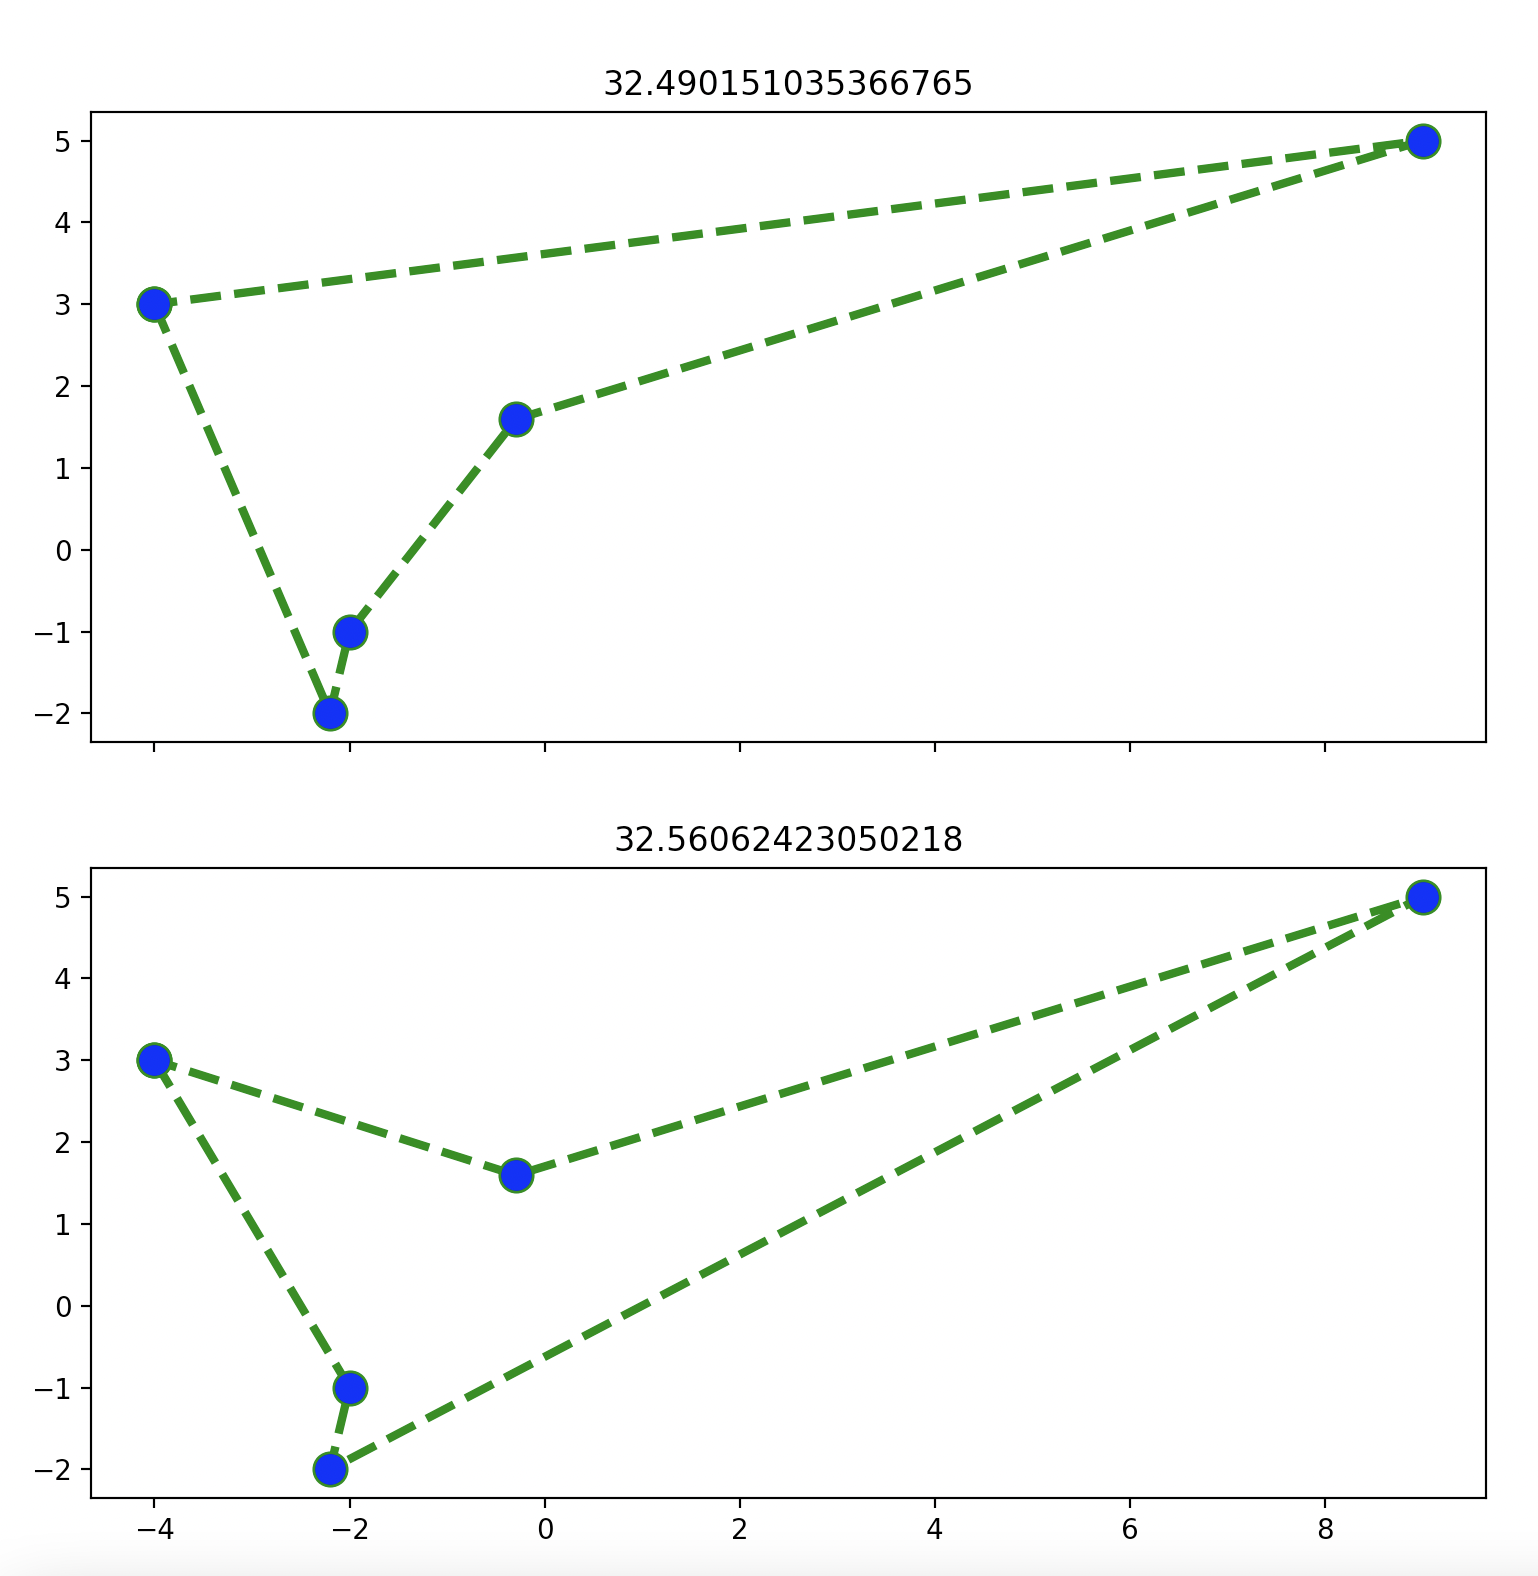
\includegraphics[width=\textwidth, height=.5\textheight, keepaspectratio]{images/5points.png}
	\caption{A Euclidean graph with 5 vertices in which the second-best TSP (bottom) shares only one edge in common with the optimal TSP (top)}\label{5points}
\end{figure}

Another interesting graph comes from the idea of the near-parallel lines mentioned in Rothe \cite{rothe1988two}. The example in \autoref{9points} shows 3 near parallel lines each made of 3 points, and the first and second-best solutions differ by 3 edges. 

\begin{figure}[!ht]
	\centering
	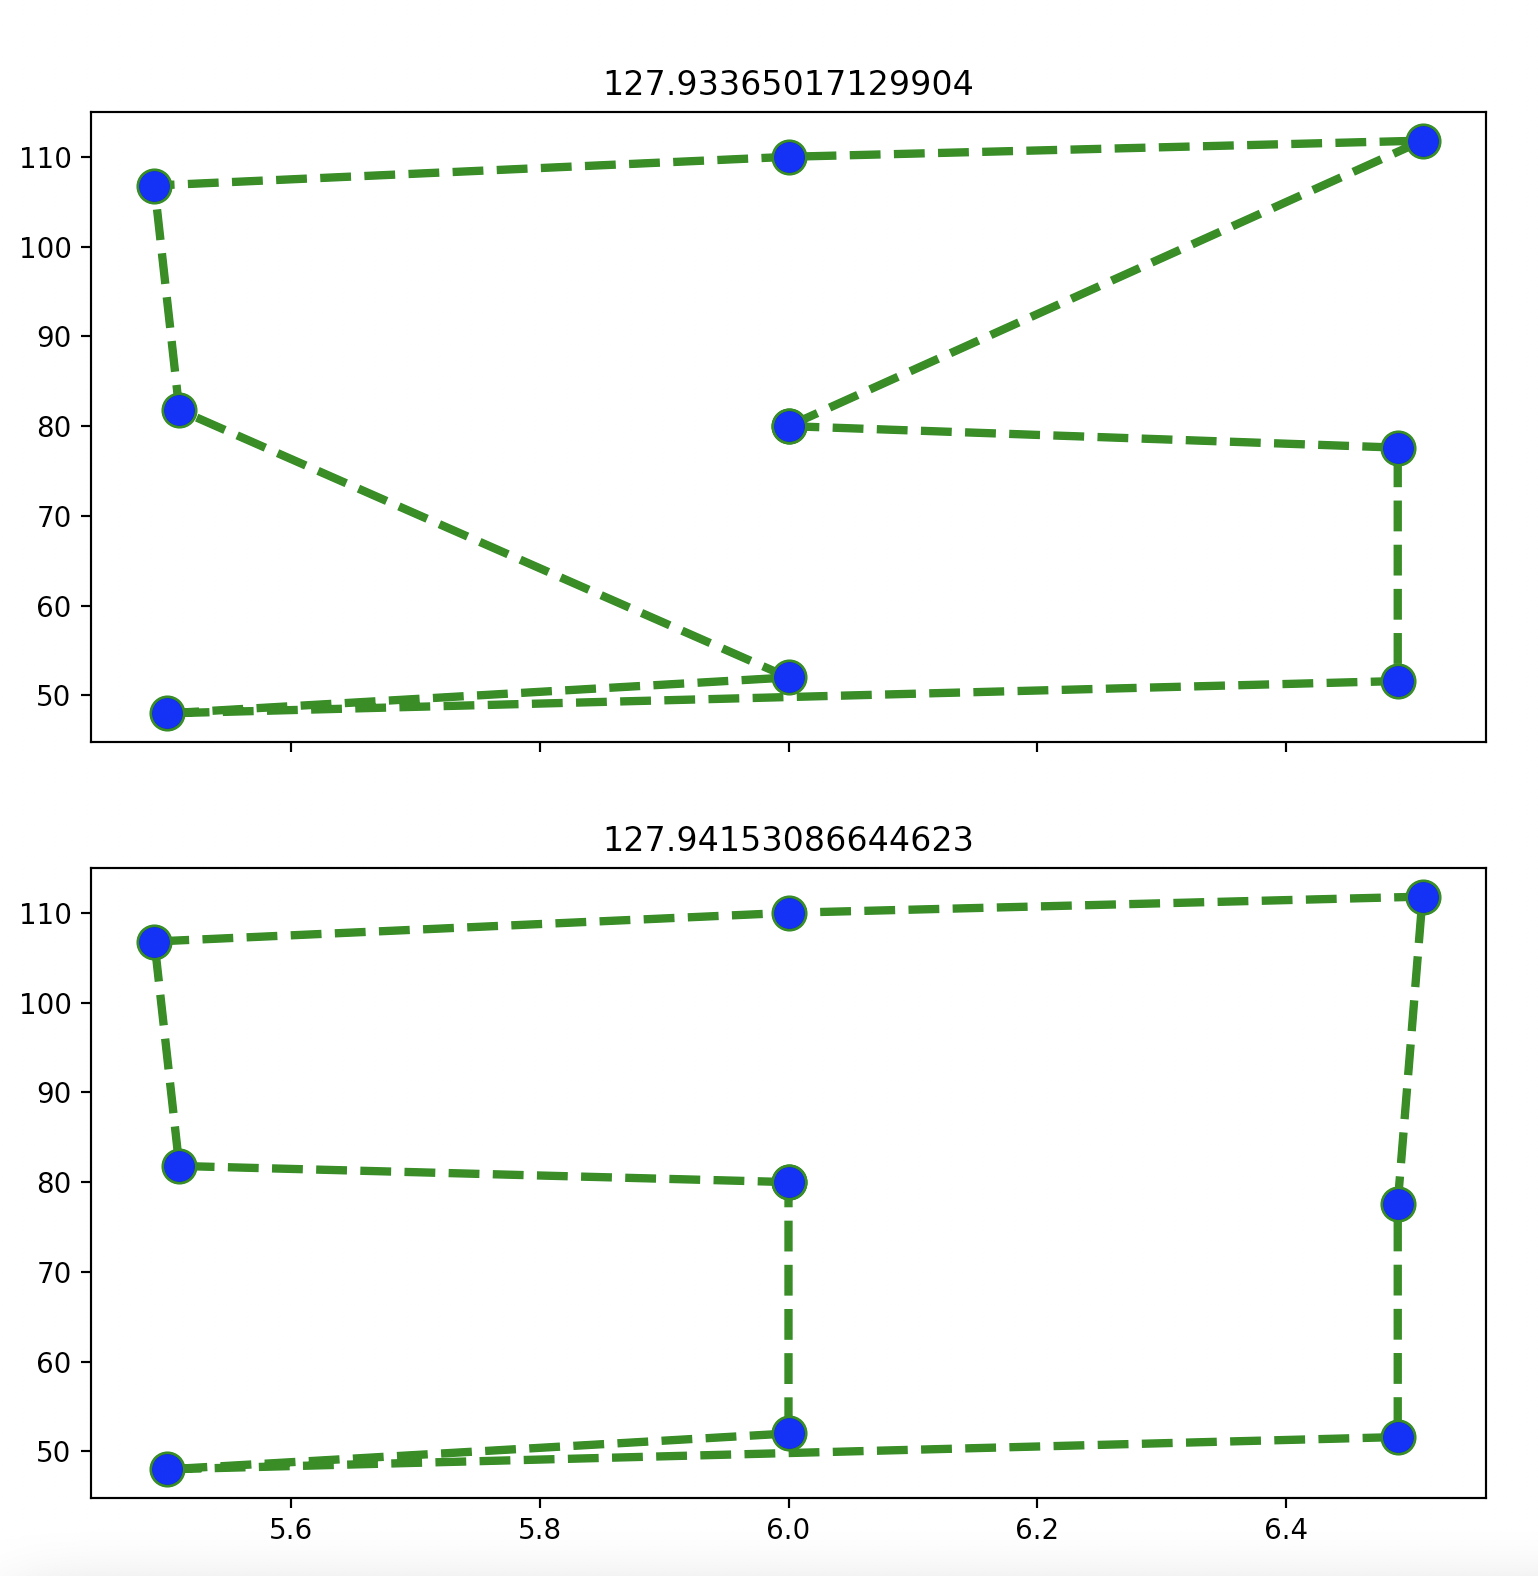
\includegraphics[width=\textwidth, height=.5\textheight, keepaspectratio]{images/9points.png}
	\caption{A Euclidean graph of 3 near-parallel lines with 9 vertices in which the second-best TSP (bottom) differs by 3 edges ($\frac{|V|}{3}$) from the optimal solution (top).}\label{9points}
\end{figure}


We will leave formalizing the second-best Euclidean TSP proofs for future work in the field, however it follows from Papadimitriou's proof of the $\npc{}$ nature of the Euclidean TSP \cite{papadimitriou1977euclidean}. In his proof, he reduces from the $\npc{}$ Exact Cover problem in which the input is a universe set $U$ and a collection of subsets $\mathcal{S}$ of $U$ and the goal is to find a subcollection $\mathcal{C} \subseteq \mathcal{S}$ in which every element in $U$ is contained in exactly one subset of $\mathcal{C}$. By creating a very specific set of Euclidean subgraphs, he is able to force a minimum Hamiltonian cycle of a certain weight if and only if there is an exact cover of the input set.

Our modification to this proof would be relatively simple compared to the proof itself. Originally, Papadimitriou uses his construction to prove that Euclidean path-TSP, rather than cycle, is NP-Complete. To show that the Euclidean tour-TSP, what we would refer to simply as Euclidean TSP, is $\npc{}$, he connects the start and endpoint with his 1-chain construction to force an optimal solution to go directly from the latter back to the former at the end of the loop. Instead, for \inob{}-Euclidean-TSP we would connect the start and endpoint with his 2-chain construction, giving two equally weighted loops that are the same besides the mode of traversal between the start and endpoint. For \exob{}-Euclidean-TSP, we would do the same, except make one of the modes through the chain a tiny amount worse than the other by moving one of its vertices a small amount to the side. For more details, it is important to read \cite{papadimitriou1977euclidean}. We would expect future work in the field to formalize this proof.


\section{Convex Euclidean TSP}
We will examine one more version of the travelling salesman problem. After it became clear that the other versions of TSP were consistently $\nph{}$, we decided to consider a much heavier restriction on the input graphs than any of the previous problems. In fact, Convex Euclidean TSP is so heavily restricted that the original optimization problem is in P, making it the first problem in the class of P that we examined that was not already studied in terms of second-best solutions. However, the easiness of the original problem does not make the second-best question uninteresting, as it is not immediately apparent whether it will still be easy to find the second-best solution as well. This type of question, asking whether or not computing the optimal solution is actually easier to find than any that come after it, is the basis behind much of the research into $k$-best problems that came before us, but is even more prevalent here as the convex Euclidean version of the travelling salesman problem feels so close to being $\nph{}$. First, let us define what we mean for a graph to be convex. If $G$ is a 2-dimensional Euclidean graph -- as defined in the section above -- in which the points form a convex polygon, then we will show that \exob{}-Convex-Euclidean-TSP and \inob{}-Convex-Euclidean-TSP on $G$ can be solved in polynomial time.  Note the known result that the optimal solution to the traveling salesman problem on a convex Euclidean graph is simply the convex hull of the graph, which is obtainable in polynomial time. This result comes from the proof that the solution to Euclidean TSP must never have crossings, which in the convex case, leads to only a single possible solution (for general Euclidean TSP, there are many non-crossing tours) \cite{quintas1965on, arora1998polynomial}.

First, we will show that the \exob{} and \inob{} versions of the problem are equivalent, assuming we ignore simple loop reversals (allowing loop reversals simply makes \inob{} very easy, as we can always reverse the best solution, whereas \exob{} would remain unchanged). 
\begin{lemma*}
        $T$ is a solution to \inob{}-Convex-Euclidean-TSP $\iff$ $T$ is a solution to \exob{}-Convex-Euclidean-TSP
\end{lemma*}
\begin{proof}
    This proof follows directly from the original proof that Convex-Euclidean-TSP is easy. Any solution other than the convex hull of the graph must have an edge crossing, and any solution with an edge crossing must have a higher total weight than a solution with no edge crossings. Since there is only one convex hull (up to rotation and reversal), this implies that any non-optimal solution is strictly worse than the optimal. Thus, if $T$ is a solution to \inob{}-Convex-Euclidean-TSP, $T$ is a solution to \exob{}-Convex-Euclidean-TSP and vice-versa.
\end{proof}
Thus, we only need to show that one of the two versions are hard, and we will have a proof that all three versions of the second-best problem are hard. We will use a proof by induction on the number of edges different between optimal tour $T$ and any other tour $T'$. Our goal is to show that any tour $T'$ can always be improved by exchanging edges with $T$. We represent tours in ``vertex,edge,vertex...,vertex" edge notation, as in $a_1,a_1a_2,a_2,...,a_na_1,a_1$ but abuse the notation to refer to only the edges in one tour that are not in the other as $T_1 \setminus T_2$.

\begin{theorem}
    Any suboptimal tour $T'$ can be altered to become $T''$ such that $w(T'') \leq w(T')$ exclusively by removing edge crossings in $T'$.
\end{theorem}

\begin{proof}
    
\textbf{\textit{(Base cases):}} \newline
\textbf{\textit{(Case 0 edge crossings):}}

If there are 0 edge crossings within $T'$, then $T' = T$ since the optimal solution to Euclidean TSP is the only solution that has no edge crossings.
\newline\textbf{\textit{(Case 1 edge crossing):}}

If there is 1 edge crossing within $T'$, let the crossing edges be $uv$ and $xy$. Due to the convexity of the graph, we can replace $uv$ and $xy$ with either $ux$ and $vy$ or $uy$ and $vx$, whichever pair doesn't cross. This replacement does not increase the total cost due to the triangle inequality, as shown in \cite{quintas1965on}. After this replacement, we have a new tour $T''$ with 0 edge crossings, which is the optimal tour $T$. This implies that $|T \setminus T'| = 2$, there are exactly two edges in $T'$ that are not in $T$.
\newline\textbf{\textit{(Inductive Step):}} Suppose that for any Hamiltonian cycle $T'$ with $k$ edge crossings within itself, we can improve $T'$ by replacing crossing edges. We will show that this must also hold for a tour $T'$ with $k+1$ edge crossings.

Let $T'$ be a tour with $k+1$ edge crossings within itself. Choose any pair of crossing edges $uv$ and $xy$. As in the base case with 1 crossing, we can replace these edges with either $ux$ and $vy$ or $uy$ and $vx$, whichever pair doesn't cross, without increasing the total cost. This replacement must always yield a new tour $T''$ with at most $k$ edge crossings. By the inductive hypothesis, we can improve $T''$ -- or at least not make it worse -- by replacing crossing edges until we reach the optimal tour $T$. Since this process is not immediately intuitive, we include an example graph in \autoref{3diff}.

\begin{figure}[!ht]
	\centering
	\begin{tikzpicture}
	    \foreach \i in {1,2,...,9}
		\node[circle, draw] (\i) at ({\i*40}:2) {\i};
	    \draw (1) -- (2);
	    \draw (2) -- (3);
	    \draw (3) -- (4);
	    \draw (4) -- (5);
	    \draw (5) -- (6);
	    \draw (6) -- (7);
	    \draw (7) -- (8);
	    \draw (8) -- (9);
	    \draw (9) -- (1);
	\end{tikzpicture} 
	\begin{tikzpicture}
	    \foreach \i in {1,2,...,9}
		\node[circle, draw] (\i) at ({\i*40}:2) {\i};
		
	    \draw (1) -- (2);
	    \draw (2) -- (4);
	    \draw (3) -- (7);
	    \draw (4) -- (5);
	    \draw (5) -- (6);
	    \draw (6) -- (7);
	    \draw (3) -- (8);
	    \draw (8) -- (9);
	    \draw (9) -- (1);
	\end{tikzpicture}
	\begin{tikzpicture}
	    \foreach \i in {1,2,...,9}
		\node[circle, draw] (\i) at ({\i*40}:2) {\i};
		
	    \draw (1) -- (2);
	    \draw (3) -- (4);
	    \draw (2) -- (7);
	    \draw (4) -- (5);
	    \draw (5) -- (6);
	    \draw (6) -- (7);
	    \draw (3) -- (8);
	    \draw (8) -- (9);
	    \draw (9) -- (1);
	\end{tikzpicture}
	\caption{An example of the original best tour $T$ (left), a tour $T'$ with $|T \setminus T'| = 3$ (middle), and an example of a tour converted from two edge crossings to one, and $|T \setminus T'| = 3$ to $|T \setminus T'| = 2$ (right)} \label{3diff}
\end{figure}

From our work above, we know that for any suboptimal tour $T'$, we can improve it by repeatedly replacing crossing edges within the tour until we reach the optimal tour $T$. If we stop the process when there is one crossings left, we will have a tour $T''$ such that $|T \setminus T''| = 2$. Since any further decrease in edge crossings would lead to simply finding the optimal solution, that implies that any second-best solution must have $|T \setminus T''| = 2$. Since the number of edges in a complete undirected graph is $\frac{|V|*(|V|-1)}{2}$, that means the number of pairs of edges is 
\begin{equation*}
    \binom{\frac{|V|*(|V|-1)}{2}}{2} = \frac{1}{2}(\frac{|V|*(|V|-1)}{2})(\frac{|V|*(|V|-1)}{2} - 1)
\end{equation*}
which is polynomial in the number of vertices. Thus, finding the second-best tour can be done in polynomial time. We can simply loop through all pairs of edges and check the total weight of a tour that includes those two edges instead of the normal ones in $T$. To determine which edges must be removed for in each case, we can simply also loop through all pairs of edges in $T$, which is $|V|*|V-1|$, and check whether that edge swap would result in a valid Hamiltonian cycle and if it was the best replacement to make. Thus, the total running time of this algorithm is $O(|V|^6)$, which, while a very large polynomial, is still polynomial. Thus, the \exob-Euclidean-Convex-TSP is in complexity class P, as are \inob{}-Euclidean-Convex-TSP and of course \exb{}-Euclidean-Convex-TSP.\end{proof}
There are clearly many ways to improve this algorithm and this solution seems hardly better than brute-force. However, our goal for now was simply to prove that the problem was solvable in polynomial time. We suspect that future work in the area can bring this complexity down to at $O(|V|^2)$ or maybe even $O(|V|)$, making it much more usable in real-world applications. Additionally, this result begs the question of what happens to the complexity of the problem with higher values of $k$ than 2? We suspect that, for a polynomial $k$, it should still be polynomial to find the $k$-th best solution following the same logic as above, since it should have at most $k$ edge-crossings. However, we will leave the proof of this to further research.





% The Traveling Salesman Problem, or TSP is a widely studied {NP-Hard} combinitorial optimization problem in which the decision version of the problem is {{NP-Hard}}. There are three commonly referenced versions of the problem.
% \section{Euclidean TSP}
% \subsection{Standard Euclidean TSP}
% \hfill\\
% If we restrict the traveling salesman problem to exist only on the Euclidean plane, or in other words, every 'city' is a point on the 2D Euclidean plane and every 'route' between two cities is the Euclidean distance between the two points, we are able to slightly limit the likely solution set. This leads to interesting results in general with Euclidean TSP, including that it permits a polynomial time approximation scheme, or an approximation algorithm with arbitrary accuracy. However, despite this approximability, Euclidean TSP is still hard in all second-best forms. In other words, it is \exobht{}, \inobht{}, and of course therefor \exbht{} and \inbht{}. This is the last time we will explicitly mention a problem being \exbht{} and \inbht{}, as any \exobht{} or \inobht{} problem must also be \exbht{} and \inbht{}, and any {NP-Hard} problem is also \exbht{} and \inbht{}. We also develop some geometric intuition for why this may be the case using example graphs.
% \subsection{Convex Shape TSP}
% \hfill\\
% If we further restrict the input graph for the problem to be a convex shape on the Euclidean plane, or in other words the input graph could be represented as a convex polygon, then the problem becomes easier. It is previously proven that finding the optimal (first best) solution for this problem is in {P}. However, it is not obvious that \exobt{{-Convex-TSP}} or \inobt{{-Convex-TSP}} are quite as easy. We prove both in our results section. 
% \section{Metric TSP}
% If instead of the Euclidean distance metric being the restriction of route costs, we use a generic metric that satisfies the triangle inequality, TSP becomes even more difficult. In this case, we lose the polynomial-time-approximation scheme, but it is still possible to create a polynomial-time approximation that is slightly better than a 3/2 approximation. Similarly to the Euclidean case, Metric TSP is both \exobht{} and \inobht{}.
% \section{General TSP}
% In the case where there are no restrictions on the cost to travel between two cities, the traveling salesman problem becomes much harder. In this case, there are no approximations with constant or arbitrary accuracy. Unsurprisingly, the general Traveling Salesman Problem is \exobht{} and \inobht{}.
\chapter{Examining Other NP-Hard Problems}
In this section, we present our proofs for the hardness of various combinatorial optimization problems in the context of finding the second-best solution.

\section{Bin Packing}
\begin{definition}[Bin Packing]
Given a bin capacity $B$, and a set of items $I$ with sizes $s(i) \in (0, B]$ for each $i \in I$, find a partition of $I$ into the minimum number of subsets (bins) such that the total size of items in each subset does not exceed $B$.
\end{definition}
While we have defined the bin packing problem above as having as output a partition of $I$, most definitions of the problem will actually simply require a solution in the form of an integer representing the minimum number of bins necessary to hold all of the items. This leads to very different results for our second-best problems, so we include both versions.
\subsection{Output is Integer $K$}
\begin{definition}[\exob{}-Bin-Packing-K]
Given an instance of the Bin Packing problem and the optimal number of bins $K$, find a packing that uses $K' > K$ bins, such that no packing with $K''$ exists such that $ K < K'' < K'$.
\end{definition}

\begin{theorem}
\exob{}-Bin-Packing-K is in $\pp{}$.
\end{theorem}
\begin{proof}
To find the second-best solution for \exob{}-Bin-Packing-K, we can simply return $K+1$, where $K$ is the optimal number of bins provided as input. This can be done in constant time, making the problem easy.
\end{proof}

\begin{definition}[\exb{}-Bin-Packing-K]
Given an instance of the Bin Packing problem, find a packing that uses $K'$ bins, such that $K' > K$, where $K$ is the optimal number of bins, and no packing with $K < K'' < K'$ bins exists.
\end{definition}

\begin{theorem}
\exb{}-Bin-Packing-K is $\nph{}$.
\end{theorem}
\begin{proof}
We can reduce the original Bin Packing problem to \exb{}-Bin-Packing-K. Given an instance of Bin Packing, we can solve \exb{}-Bin-Packing-K and return the result minus one as the solution to the original problem. Since Bin Packing is NP-Hard, and thus calculation can be done in constant time, \exb{}-Bin-Packing-K is also $\nph{}$.
\end{proof}

\begin{definition}[\inob{}-Bin-Packing-K]
Given an instance of the Bin Packing problem, find a packing that uses $K'$ bins, such that $K' \geq K$, where $K$ is the optimal number of bins, and no packing with $K \geq K'' < K'$ bins exists.
\end{definition}

\begin{theorem}
\inob{}-Bin-Packing-K is undefined.
\end{theorem}
As is sometimes the case for the inclusive variety of 2nd-Best problems, this problem does not permit a clear definition of an inclusive second-best solution, as the solution is just an integer, not an object that can have a cost attached to it but is itself distinct from said cost. Thus, we can consider \inob{}{-Bin-Packing-K} either equivalent to the \exob{} variety, or entirely undefined. In general, when this occurs, we will call the problem undefined rather than attempting to force it into a strange definition. \newline

\subsection{Output is Partition $P$}
\begin{definition}[\exob{}-Bin-Packing-P]
Given an instance of the Bin Packing problem and an optimal partition $P$ of items into bins, find a partition $P'$ that uses $|P'| > |P|$ bins, such that no partition with $|P| < |P''| < |P'|$ bins exists.
\end{definition}

\begin{theorem}
\exob{}-Bin-Packing-P is in $\pp{}$.
\end{theorem}
\begin{proof}
To find the second-best solution for \exob{}-Bin-Packing-P, we can take the optimal partition $P$ provided as input and move one item from any bin to a new bin. This new partition is a valid second-best solution and can be found in polynomial time.
\end{proof}

\begin{definition}[\inob{}-Bin-Packing-P]
Given an instance of the Bin Packing problem and an optimal partition $P$ of items into bins, find a partition $P' \neq P$ that uses $|P'| \geq |P|$ bins, such that no partition $P'' \neq P$ with $|P| \leq |P''| < |P'|$ bins exists.
\end{definition}
\begin{theorem}
\inob{}{-Bin-Packing-P} is $\nph{}$.
\end{theorem}
\begin{proof} 
We introduce the Partition Problem, a known $\npc{}$ problem.
\begin{definition}[Partition]
    Given a multiset $S$ of positive integers, find two disjoint subsets $S_1$ and $S_2$ such that $S = S_1 \cup S_2$ and $sum(S_1) = sum(S_2)$.
\end{definition}
We will reduce the Partition problem to \inob{}-Bin-Packing-P.

Given an instance of the Partition problem with a multiset $S = \{a_1, a_2, \ldots, a_n\}$, we construct an instance of \inob{}-Bin-Packing-P as follows:
\begin{enumerate}
    \item Create a set of items $I = \{x_1, x_2, ..., x_n, y_1, y_2\}$, where $s(x_i) = a_i$ for $1 \leq i \leq n$, and $s(y_1) =s(y_2) = \frac{1}{2} \sum_{i=1}^n a_i$.
    \item Set the bin capacity to $B = \sum_{i=1}^n a_i$.
    \item Set the optimal partition $P = \{\{y_1, y_2\}, I - \{y_1, y_2\}\}$. 
\end{enumerate}
First, note that every step of this construction is easily completed in polynomial time on the size of the input for the Partition problem.
Now, we argue that the constructed instance of \inob{}-Bin-Packing-P has a second-best partition $P'$ with $|P'| = |P|$ if and only if the original Partition instance has a solution. 

$(\Rightarrow)$ Suppose the constructed \inob{}-Bin-Packing-P instance has a second-best partition $P'$ with $|P'| = |P|$. Since $P'$ must be different from $P$ and $|P'| = 2$, it must partition the items in $I - \{y_1, y_2\}$ into two bins. Thereore, we can say $P' = \{S_1 \cup \{y_1\}, S_2 \cup \{y_2\}\}$ (we assign $y_1$ and $y_2$ without loss of generality, because clearly any partition in which they are in the same set will be exactly $P$). As $P'$ is a valid solution to the Bin Packing problem, the sum of item sizes in each bin must not exceed the bin capacity $B$. However, since the total sum of all items in $I$ is $2B=2\sum_{i=1}^{n}a_i=$, this can only be possible if each side has sum $B=\sum_{i=1}^{n}a_i$. As we noted, $y_1$ and $y_2$ are in different sets in the partition, and each have sizes of $\frac{B}{2}$. Thus, $S_1$ and $S_2$ must each sum to $\frac{B}{2} = \frac{1}{2}\sum_{i=1}^{n}a_i$ and thus form a solution to the original Partition instance.

$(\Leftarrow)$ Suppose the original Partition instance has a solution, i.e., there exist subsets $S_1$ and $S_2$ such that $S_1 \cup S_2 = S$ and $\sum_{a_i \in S_1} a_i = \sum_{a_i \in S_2} a_i = \frac{1}{2} \sum_{i=1}^n a_i$. We can construct a second-best partition $P'$ for the \inob{}-Bin-Packing-P instance as follows: $P' = \{\{x_i : a_i \in S_1\} \cup \{y_1\}, \{x_i : a_i \in S_2\}\cup\{y_2\}\}$. By construction, $P'$ is a valid partition with $|P'| = |P|$ and $P' \neq P$.

Since the Partition problem is $\nph{}$ and we have shown a polynomial-time reduction from Partition to \inob{}-Bin-Packing-P, we can conclude that \inob{}-Bin-Packing-P is also $\nph{}$.
\end{proof}

\begin{definition}[\exb{}-Bin-Packing-P]
Given an instance of the Bin Packing problem, find a partition $P'$ that uses $|P'|$ bins, such that $|P'| > |P|$, where $P$ is an optimal partition, and no partition $P''$ with $|P| < |P''| < |P'|$ bins exists.
\end{definition}
\begin{theorem}
\exb{}-Bin-Packing-P is $\nph{}$.
\end{theorem}
\begin{proof}
The proof that \exb{}-Bin-Packing-P is NP-hard follows essentially the same process as our proof that \inob{}-Bin-Packing-P is $\nph{}$. The only difference we would need to include would be that \exb{}-Bin-Packing would not be provided with the optimal solution and would return a partition of size three if the partition problem has a solution. This is because that implies by the definition of the exclusive version that the actual best solution has to be better than three, meaning there is a solution that includes two or less bins. From the same logic as above, this directly implies the original partition problem has a solution. Thus, \exb{}-Bin-Packing-P is $\nph{}$.


\end{proof}



\section{Maximum Clique}

\begin{definition}[Maximum Clique]
Given a graph $G = (V, E)$, find a maximum-size subset $C \subseteq V$ such that for every pair of vertices $u, v \in C$, $(u, v) \in E$. That is, $C$ is the set of vertices in the largest completely connected subgraph of $G$. 
\end{definition}
Similarly to Bin Packing, there are two possible formulations of the Maximum Clique second best problems. In this case, we can consider the standard Max-Clique problem, but we can also consider ``Maximum Maximal Clique". A maximal clique is a subset of completely connected vertices in $G$ such that no additional vertices in $G$ could be added to the subset and still have it be a clique. In other words, there are no ``easy" additions to the clique, it would take more than a single pass checking the vertices and their neighbors to find a better clique. Finding the maximum of all these maximal cliques is typically the same as finding the simple maximum, but when looking for the second best, it does change the solution, and the hardness of the probem. We begin with the version that does not require maximality.
\subsection{Maximum Clique}
\begin{definition}[\exob{}-Max-Clique]
Given an instance of the Maximum Clique problem and an optimal clique $C$, find a clique $C'$ such that $|C'| < |C|$ and no clique $C''$ with $|C'| < |C''| < |C|$ exists.
\end{definition}

\begin{theorem}
\exob{}-Max-Clique is in $\pp{}$.
\end{theorem}
\begin{proof}
To find the second-best solution for \exob{}-Max-Clique, we can take the optimal clique $C$ provided as input and remove any vertex from $C$ to create a new clique. This new clique is a valid second-best solution and can be found in polynomial time.
\end{proof}

\begin{definition}[\inob{}-Max-Clique]
Given an instance of the Maximum Clique problem and an optimal clique $C$, find a clique $C' \neq C$ such that $|C'| \leq |C|$ and no clique $C'' \neq C$ with $|C'| \leq |C''| < |C|$ exists.
\end{definition}
\begin{theorem}
\inob{}-Max-Clique is $\nph{}$.
\end{theorem}

\begin{proof}
    This proof parallels the original proof that showed the $\nph{}$ nature of Maximum Clique. We will reduce from the problem Karp used to introduce the concept of $\nph{}$ness in the first place, the Satisfiability problem, or SAT. First, let us define this problem. 
    \begin{definition}[Satisfiability (SAT)]
Given a Boolean formula $\phi$ in conjunctive normal form (CNF), represented as a set of clauses $D = \{c_1, c_2, \ldots, c_m\}$ over a set of variables $X = \{x_1, x_2, \ldots, x_n\}$, where each clause $c_i$ is a disjunction of literals (variables or their negations), determine whether there exists an assignment of truth values to the variables such that the formula $\phi$ evaluates to true. As an example, a boolean formula $\phi$, could be $\phi = (x_1 \vee x_2 \vee \neg x_3) \wedge (x_3) \wedge (\neg x_1 \vee \neg x_2)$. This formula is satisfiable, since we could use the variable assignment
$\begin{pmatrix}
    x_1 \\
    x_2 \\
    x_3
\end{pmatrix} =
\begin{pmatrix}
    0 \\
    1 \\
    1
\end{pmatrix}.$
\end{definition}
We take the input on SAT, $\phi$, and create an input, $G = (V, E)$ for \inob{}-Max-Clique as follows:
\begin{enumerate}
    \item For every clause $d \in D$, and every literal $a$ which is either a variable in $X$ or the negation of a variable in $X$, we create a vertex $(d, a)$.
    \item We create an edge $e$ between two vertices, $(d_1, a_1)$ and $(d_2, a_2)$, if $d_1 \neq d_2$ and $a_1 \neq a_2$.
    \item We also create a set of $m$ additional vertices $C =\{v_1, ..., v_m\}$ and add an edge between every pair of $v_i \neq v_j$.
\end{enumerate}
Each of these steps can easily be implemented in polynomial time.

We show that providing this graph as input to \inob{}-Max-Clique along with optimal clique $C$ must solve our SAT instance. In particular, if \inob{}-Max-Clique is able to find another clique of size $m$, then our SAT instance must be satisfiable. Otherwise, it must not be satisfiable. Every step above is clearly polynomial in the size of the input for the original SAT instance.

First, we must show that $C$ with size $m$ is a maximum clique. Firstly, it is by our definition a clique, as every vertex in $C$ is connected. For optimality, any clique containing a vertex of the form $(d, a)$ cannot include another vertex $(d', a')$ where either $d = d'$ or $a = a'$, as there are no edges between such pairs of vertices. Therefore, any clique containing vertices of the form $(d, a)$ can have at most one vertex per clause, resulting in a clique of size at most $m$. Thus, the optimal clique in $G$ has size exactly $m$.

$(\Rightarrow)$ Suppose the \inob{}-Max-Clique instance has a second-best clique $C'$ with $|C'| = |C|$, where $C$ is the optimal clique. We claim that the SAT instance is satisfiable. Since $C' \neq C$ and there are no edges between the vertices in $C$ and the remainder of $G$, $C'$ must contain exclusively vertices of the form $(d, a)$. For each variable $x_i$, if $C'$ contains a vertex $(d, x_i)$, set $x_i$ to true. Otherwise, if $C'$ contains a vertex $(d, \neg x_i)$, set $x_i$ to false. If $C'$ does not contain any vertex corresponding to $x_i$ or $\neg x_i$, assign $x_i$ arbitrarily. This assignment satisfies the SAT instance because for each clause $d$, at least one of its literals must be true and since $C'$ is a clique of size $m$ and cannot contain vertices with conflicting literals, it contains at most one variable from each clause. Therefore, the clique effectively contains one true literal for each clause, showing that such an assignment must be possible.

$(\Leftarrow)$ Suppose the SAT instance is satisfiable. Let $A$ be a satisfying assignment for $\phi$. We can construct a second-best clique $C'$ for the \inob{}-Max-Clique instance as follows: for each clause $d$, select a literal $a$ that is true under the assignment $A$ and add the corresponding vertex $(d, a)$ to $C'$. By construction, $C'$ is of size $|C'| = m = |C|$, and $C' \neq C$ since it contains exclusively vertices of the form $(d, a)$ instead of $\{v_1, ..., v_m\}$. Let two vertices selected by this algorithm be $x_1 = (d_1, a_1), x_2 = (d_2, a_2)$. Assume towards a contradiction that $x_1$ and $x_2$ are not neighbors in the input graph. That means either $d_1 = d_2$ or $a_1 = \neg a_2$. Since the algorithm iterated over the clauses selecting only one literal from each, $d_1 \neq d_2$. However, since we select only a true literal from each clause, that means both $a_1$ and $a_2$ are true. However, if one is the negation of the other, that would be impossible. Therefore, by contradiction, $x_1$ and $x_2$ must be neighbors and therefore $C'$ is a clique of size $|C|$.

Since SAT is $\nph{}$ and we have shown a polynomial-time reduction from SAT to \inob{}-Max-Clique, we can conclude that \inob{}-Max-Clique is also $\nph{}$.

\end{proof}

\begin{definition}[\exb{}-Max-Clique]
Given an instance of the Maximum Clique problem, find a clique $C'$ such that $|C'| < |C|$, where $C$ is an optimal clique, and no clique $C''$ with $|C'| < |C''| < |C|$ exists.
\end{definition}
\begin{theorem}
    \exb{}-Max-Clique is $\nph{}$.
\end{theorem}
\begin{proof}
    This proof is nearly the same as the previous proof, except in this case we create an optimal clique of size $m+1$ and don't supply it to the subproblem. This simple conversion is not possible for all problems, and in coming to this proof we did not originally formulate them the same way. For these reasons and to be absolutely rigourous, the proof can be described as follows:
 We will reduce from the Satisfiability problem, or SAT, as defined earlier.

We take the input on SAT, $\phi$, and create an input, $G = (V, E)$, for \exb{}-Max-Clique. 
\begin{enumerate}
    \item For every clause $d \in D$, and every literal $a$ which is either a variable in $X$ or the negation of a variable in $X$, we create a vertex $(d, a)$.
    \item We create an edge $e$ between two vertices, $(d_1, a_1)$ and $(d_2, a_2)$, if $d_1 \neq d_2$ and $a_1 \neq a_2$. 
    \item We also create a set of $m+1$ vertices $C =\{v_1, ..., v_{m+1}\}$ and add an edge between every pair of $v_i \neq v_j$. 
\end{enumerate} 
All of these steps can be completed in polynomial time.
We now show that providing this graph as input to \exb{}-Max-Clique must solve our SAT instance. In particular, if \exb{}-Max-Clique is able to find a clique of size $m$, then our SAT instance must be satisfiable. Otherwise, it must not be satisfiable. Importantly, every step in the above process is clearly polynomial in the size of the SAT input.

First, we must show that $C$ with size $m+1$ is a maximum clique. Firstly, it is by our definition a clique, as every vertex in $C$ is connected. For optimality, any clique containing a vertex of the form $(d, a)$ cannot include another vertex $(d', a')$ where either $d = d'$ or $a = a'$, as there are no edges between such pairs of vertices. Therefore, any clique containing vertices of the form $(d, a)$ can have at most one vertex per clause, resulting in a clique of size at most $m$. Thus, the vertices that are instead of the form $\{v_1, ..., v{m+1}\}$ must compose the optimal clique in $G$, as of course they have size exactly $m+1$.

$(\Rightarrow)$ Suppose the \exb{}-Max-Clique instance has a second-best clique $C'$ with $|C'| = m$. We claim that the SAT instance is satisfiable. Since $C' \neq C$ and there are no edges between the vertices in $C$ and the remainder of $G$, $C'$ must contain exclusively vertices of the form $(d, a)$. For each variable $x_i$, if $C'$ contains a vertex $(d, x_i)$, set $x_i$ to true. Otherwise, if $C'$ contains a vertex $(d, \neg x_i)$, set $x_i$ to false. If $C'$ does not contain any vertex corresponding to $x_i$ or $\neg x_i$, assign $x_i$ arbitrarily. This assignment satisfies the SAT instance because for each clause $d$, at least one of its literals must be true and since $C'$ is a clique of size $m$ and cannot contain vertices with conflicting literals, it contains at most one variable from each clause. Therefore, the clique effectively contains one true literal for each clause, showing that such an assignment must be possible

$(\Leftarrow)$ Suppose the SAT instance is satisfiable. Let $A$ be a satisfying assignment for $\phi$. We can construct a second-best clique $C'$ for the \exb{}-Max-Clique instance as follows: for each clause $d$, select a literal $a$ that is true under the assignment $A$ and add the corresponding vertex $(d, a)$ to $C'$. By construction, $C'$ is of size $|C'| = m < |C|$. Let two vertices selected by this algorithm be $x_1 = (d_1, a_1), x_2 = (d_2, a_2)$. Assume towards a contradiction that $x_1$ and $x_2$ are not neighbors in the input graph. That means either $d_1 = d_2$ or $a_1 = \neg a_2$. Since the algorithm iterated over the clauses selecting only one literal from each, $d_1 \neq d_2$. However, since we select only a true literal from each clause, that means both $a_1$ and $a_2$ are true. However, if one is the negation of the other, that would be impossible. Therefore, by contradiction, $x_1$ and $x_2$ must be neighbors and therefore $C'$ is a clique of size $m$.

Since SAT is $\nph{}$ and we have shown a polynomial-time reduction from SAT to \exb{}-Max-Clique, we can conclude that \exb{}-Max-Clique is also $\nph{}$.
\end{proof}

\subsection{Maximum Maximal Clique}
\begin{definition}[\exob{}-Max-Maximal-Clique]
Given an instance of the Maximum Clique problem and an optimal clique $C$, find a maximal clique $C'$ such that $|C'| < |C|$ and no maximal clique $C''$ with $|C'| < |C''| < |C|$ exists.
\end{definition}

\begin{theorem}
\exob{}-Max-Maximal-Clique is $\nph{}$.
\end{theorem}
\begin{proof}
We can reduce the original Maximum Clique problem to \exob{}-Max-Maximal-Clique. Given an instance of Maximum Clique, we can create a new input graph $G'$. In $G'$, we let $G$ exist as a subgraph unchanged in $G'$, but we also have another subgraph $C$ with $|V(G)| + 1$ vertices that is maximally connected. In other words, we add a clique that is one vertex larger than $G$ itself that is unconnected to the vertices in $G$. Clearly, this clique is the maximum clique in $G'$. Thus, we can create an instance of \exob{}-Max-Maximal-Clique with the input of $G'$ along with optimal solution $C$. Since any strict subgraph of $C$ in $G'$ would not be maximal (as we could simply add a missing vertex from $C$ back in), the solution to this instance on \exob{}-Max-Maximal-Clique must be the maximum maximal clique in the original $G$, which is exactly defined as the solution to the original problem. Thus, since Maximum Clique is in $\nph{}$, \exob{}-Max-Maximal-Clique is also $\nph{}$.
\end{proof}

\begin{definition}[\inob{}-Max-Maximal-Clique]
Given an instance of the Maximum Clique problem and an optimal clique $C$, find a maximal clique $C'$ such that $|C'| \leq |C|$ and no maximal clique $C'' \neq C$ with $|C'| < |C''|$ exists.
\end{definition}

\begin{theorem}
\inob{}-Max-Maximal-Clique is $\nph{}$.
\end{theorem}
\begin{proof}
We can reduce the original Maximum Clique problem to \inob{}-Max-Maximal-Clique in the exact same way as \exob{}. It is clear that the clique, $C$, we created in $G'$ for \exob{}-Max-Maximal-Clique is explicitly larger than any other possible maximal clique, making \inob{}-Max-Maximal-Clique produce the exact same result as the exclusive version. Thus, the proof for \inob{}-Max-Maximal-Clique follows directly from the proof for \exob{}-Max-Maximal
\end{proof}

\begin{definition}[\exb{}-Max-Maximal-Clique]
Given an instance of the Maximum Clique problem find a maximal clique $C'$ such that $|C'| \leq |C|$ for an optimal clique $C$ and no maximal clique $C'' \neq C$ with $|C'| < |C''|$ exists.
\end{definition}

\begin{theorem}
\exb{}-Max-Maximal-Clique is $\nph{}$.
\end{theorem}
\begin{proof}
This follows from \autoref{exbhard} we proved in an earlier section. Since \exob{}-Max-Maximal-Clique is $\nph{}$, \exb{}-Max-Maximal-Clique must also be.
\end{proof}

\section{Minimum Vertex Cover}
\begin{definition}[Minimum Vertex Cover]
Given a graph $G = (V, E)$, find a minimum-size subset $C \subseteq V$ such that for every edge $(u, v) \in E$, either $u \in C$ or $v \in C$.
\end{definition}

Much like for maximal clique, there is a second version of vertex cover that requires the vertex cover be minimal, where no vertices in $C$ can simply be removed without loss of its covering nature.
\subsection{Minimum Vertex Cover}
\begin{definition}[\exob{}-Min-Vertex-Cover]
Given an instance of the Minimum Vertex Cover problem and an optimal vertex cover $C$, find a vertex cover $C'$ such that $|C'| > |C|$ and no vertex cover $C''$ with $|C| < |C''| < |C'|$ exists.
\end{definition}

\begin{theorem}
\exob{}-Min-Vertex-Cover is in $\pp{}$.
\end{theorem}
\begin{proof}
To find the second-best solution for \exob{}-Min-Vertex-Cover, we can take the optimal vertex cover $C$ provided as input and add any vertex not in $C$ to create a new vertex cover. This new vertex cover is a valid second-best solution and can be found in polynomial (constant) time.
\end{proof}

\begin{definition}[\inob{}-Min-Vertex-Cover]
Given an instance of the Minimum Vertex Cover problem and an optimal vertex cover $C$, find a vertex cover $C' \neq C$ such that $|C'| \geq |C|$ and no vertex cover $C'' \neq C$ with $|C| \leq |C''| < |C'|$ exists.
\end{definition}

\begin{theorem}
\inob{}-Min-Vertex-Cover is $\nph{}$.
\end{theorem}
\begin{proof}
This is a noteworthy proof as it is the first time in this section that we will use a problem we previously defined to prove the hardness of a new problem. We will be reducing from \inob{}-Max-Clique to \inob{}-Min-Vertex-Cover.

Given an instance of \inob{}-Max-Clique with a graph $G = (V, E)$ and an optimal clique $C$, we construct an instance of \inob{}-Min-Vertex-Cover as follows:

Create a new graph $G' = (V', E')$ as follows:
\begin{enumerate}
    \item $V' = V$ 
    \item $E' = \{(u, v) : u, v \in V, u \neq v, (u, v) \notin E\}$. In other words, $E'$ includes every edge that is not in $E$.
\end{enumerate}
Clearly neither of these steps requires more than polynomial time on the size of the input graph to complete.

We call $G'$ the ``complement graph" of $G$.
Set the optimal vertex cover in $G'$ to $C' = V - C$.
We show that providing this graph $G'$ as input to \inob{}-Min-Vertex-Cover along with the optimal vertex cover $C'$ must solve our \inob{}-Max-Clique instance. In particular, if \inob{}-Min-Vertex-Cover is able to find another vertex cover of size $|V| - |C|$, then our \inob{}-Max-Clique instance must have a second-best clique of size $|C|$. Otherwise, it must not have such a clique. If \inob{}-Max-Clique does not have a second-best clique of size $|C|$, then it becomes equivalent to \exob{}-Max-Clique, which we have already shown to be in $P$. Additionally, note that it is very easy to construct this complement graph in polynomial time in the size of the input.

First, we must show that $C'$ with size $|V| - |C|$ is a minimum vertex cover in $G'$. By the definition of a vertex cover, every edge in $G'$ must have at least one endpoint in $C'$. Since $C$ is a clique in $G$, there are no edges between any pair of vertices in $C$ in $G'$, the complement of $G$. Therefore, $C'$ covers all edges in $G'$, making it a valid vertex cover. To prove $C'$ is optimal, suppose towards a contradiction that there exists a vertex cover $C''$ in $G'$ with $|C''| < |C'|$. Then, consider $V - C''$. Clearly, $|V-C''| > |V-C'| = |C|$, thus if this set is a clique in $G$, then it would be a larger clique than the original $C$. But, we already know $C''$ is a vertex cover in $G'$. To show that $V - C''$ is indeed a clique in $G$, suppose for the sake of contradiction that there exist two vertices $u, v \in V - C''$ such that $(u, v) \notin E$. By the construction of $G'$, this means that $(u, v) \in E'$. However, since $C''$ is a vertex cover in $G'$, at least one of $u$ or $v$ must be in $C''$, contradicting the fact that $u, v \in V - C''$. Therefore, every pair of vertices in $V - C''$ must be connected by an edge in $G$, making $V - C''$ a clique in $G$. would be a clique in $G$ with size greater than $|C|$, contradicting the optimality of $C$ in $G$. Therefore, we have proven by contradiction that there is no $C''$, a vertex cover smaller than $C'$. Thus, $C'$ is a minimum vertex cover in $G'$. Now, we must show that \inob{}-Min-Vertex-Cover finds a vertex cover with size $|C'|$ $\iff$ \inob{}-Max-Clique has a second-best clique of size $|C$. 

$(\Rightarrow)$ Suppose the \inob{}-Min-Vertex-Cover instance has a second-best vertex cover $C''$ with $|C''| = |C'|$, where $C'$ is the optimal vertex cover. We claim that $V - C''$ is a second-best clique in $G$ with size $|C|$. Since $C'' \neq C'$ and $|C''| = |C'|$, $V - C''$ must be different from $C = V - C'$ and $|V - C''| = |V| - |C''| = |V| - |C'| = |C|$. Therefore, $V - C''$ is a clique in $G$ with size $|C|$, making it a second-best clique.

$(\Leftarrow)$ Suppose the \inob{}-Max-Clique instance has a second-best clique $C''$ with $|C''| = |C|$. We claim that $V - C''$ is a second-best vertex cover in $G'$ with size $|C'|$. Since $C'' \neq C$ and $|C''| = |C|$, $V - C''$ must be different from $C'$ and $|V - C''| = |V| - |C''| = |V| - |C| = |C'|$. Since $C''$ is a clique in $G$, there are no edges between any pair of vertices in $C''$ in $G'$. Therefore, $V - C''$ covers all edges in $G'$, making it a second-best vertex cover.

Since \inob{}-Max-Clique is $\nph{}$ and we have shown a polynomial-time reduction from \inob{}-Max-Clique to \inob{}-Min-Vertex-Cover, we have shown that \inob{}-Min-Vertex-Cover is also $\nph{}$.
\end{proof}


\begin{definition}[\exb{}-Min-Vertex-Cover]
Given an instance of the Minimum Vertex Cover problem, find a vertex cover $C'$ such that $|C'| > |C|$, where $C$ is an optimal vertex cover, and no vertex cover $C''$ with $|C| < |C''| < |C'|$ exists.
\end{definition}


\begin{theorem}
\exb{}-Min-Vertex-Cover is $\nph{}$.
\end{theorem}
\begin{proof}
To prove that \exb{}-Min-Vertex-Cover is NP-hard, we will reduce from \exb{}-Max-Clique.

Given an instance of \exb{}-Max-Clique with a graph $G = (V, E)$, we construct an instance of \exb{}-Min-Vertex-Cover as follows:
reate the complement graph $G' = (V', E')$ of $G$,
\begin{enumerate}
    \item C $V' = V$ 
    \item $E' = {(u, v) : u, v \in V, u \neq v, (u, v) \notin E}$.
\end{enumerate}

We claim that the second-best clique in $G$ must be exactly $V - C$, where $C$ is the result of \exb{}-Min-Vertex-Cover on our constructed input.

Note that all of the logic from the \inob{}-Min-Vertex-Cover proof carries over here, allowing us to say that the second-best solution of the vertex cover problem is the complement of the second best solution of the clique problem. Thus, we will spare the repetitive details here.

\end{proof}
\subsection{Minimum Minimal Vertex Cover}
As mentioned above, we have a second formulation for the minimum vertex cover, where we require the solutions to the second-best problems to be minimal.
\begin{definition}[\exob{}-Min-Minimal-Vertex-Cover]
Given an instance of the Minimum Vertex Cover problem and an optimal vertex cover $C$, find a minimal vertex cover $C'$ such that $|C'| > |C|$ and no minimal vertex cover $C''$ with $|C| < |C''| < |C'|$ exists.
\end{definition}

\begin{theorem}
\exob{}-Min-Minimal-Vertex-Cover is $\nph{}$.
\end{theorem}
\begin{proof}
Given an instance of \exob{}-Max-Maximal-Clique with a graph $G = (V, E)$ and an optimal maximal clique $X$, we construct an instance of \exob{}-Min-Minimal-Vertex-Cover as follows:

\begin{enumerate}
    \item  Create the complement graph $G' = (V', E')$ of $G$, where $V' = V$ and $E' = {(u, v) : u, v \in V, u \neq v, (u, v) \notin E}$.
    \item Set the optimal minimal vertex cover in $G'$ to $C = V - X$.
\end{enumerate}
Of course, both of these procedures can easily be implemented in polynomial time on the size of the input graph. 

Let us first prove a lemma.
\begin{lemma*}
    $X$ is a maximal clique in $G$ $\iff$ $C = V - X$ is a minimal vertex cover in G'.
\end{lemma*}
\begin{proof}
Let $G = (V, E)$ be an undirected graph, and let $X \subseteq V$ be a maximal clique in $G$. We claim that $C = V - X$ is a minimal vertex cover in $G$.

First, we have already proven above that $C$ is at least a vertex cover, so we need only prove that it is minimal. 

 Let $w$ be an arbitrary vertex in $C$. We need to show that $C - {w}$ is not a vertex cover. Since $X$ is a maximal clique, there must be a vertex $z$ in $X$ such that $(w, z)$ is not an edge in $G$ (otherwise, $X \cup {w}$ would be a larger clique, contradicting the maximality of $X$). Consider the edge $(w, z)$. Since $w \in C$ and $z \in X$, neither $w$ nor $z$ is in $C - {w}$. Therefore, $C - {w}$ does not cover the edge $(w, z)$ and is not a vertex cover. Since $w$ was arbitrary, this implies that removing any vertex from $C$ results in a set that is not a vertex cover, and thus $C$ is minimal.

We have shown that $C = V - X$ is a vertex cover and that it is minimal. Therefore, the complement of a maximal clique in its complement graph is a minimal vertex cover.
\end{proof}
Now, we will show that a set $X'$ is a solution to \exob{}-Max-Maximal-Clique in $G$ if and only if $S = V - X'$ is a solution to \exob{}-Min-Minimal-Vertex-Cover in $G'$.

$(\Rightarrow)$ Suppose $X'$ is a solution to \exob{}-Max-Maximal-Clique in $G$. Then, $X'$ is a maximal clique in $G$ with $|X'| < |X|$, and no maximal clique $X''$ exists in $G$ with $|X'| < |X''| < |X|$. We claim that $S = V - X'$ is a solution to \exob{}-Min-Minimal-Vertex-Cover in $G'$. First, since $X'$ is a maximal clique in $G$, $S$ is a minimal vertex cover in $G'$. Moreover, $|S| = |V| - |X'| > |V| - |X| = |C|$, so $S$ is a minimal vertex cover larger than the optimal one. Finally, suppose there exists a minimal vertex cover $C'$ in $G'$ with $|C| < |C'| < |S|$. Then, $X'' = V - C'$ would be a maximal clique in $G$ with $|X'| < |X''| < |X|$, contradicting the assumption that $X'$ is a solution to \exob{}-Max-Maximal-Clique.

$(\Leftarrow)$ Suppose $S$ is a solution to \exob{}-Min-Minimal-Vertex-Cover in $G'$. Then, $S$ is a minimal vertex cover in $G'$ with $|S| > |C|$, and no minimal vertex cover $C'$ exists in $G'$ with $|C| < |C'| < |S|$. We claim that $X' = V - S$ is a solution to \exob{}-Max-Maximal-Clique in $G$. First, since $S$ is a minimal vertex cover in $G'$, $X'$ is a maximal clique in $G$. Moreover, $|X'| = |V| - |S| < |V| - |C| = |X|$, so $X'$ is a maximal clique smaller than the optimal one. Finally, suppose there exists a maximal clique $X''$ in $G$ with $|X'| < |X''| < |X|$. Then, $C' = V - X''$ would be a minimal vertex cover in $G'$ with $|C| < |C'| < |S|$, contradicting the assumption that $S$ is a solution to \exob{}-Min-Minimal-Vertex-Cover.

Therefore, we have shown that obtaining a solution to \exob{}-Min-Minimal-Vertex-Cover in $G'$ is equivalent to obtaining a solution to \exob{}-Max-Maximal-Clique in $G$. Since \exob{}-Max-Maximal-Clique is NP-hard (as shown earlier), \exob{}-Min-Minimal-Vertex-Cover must also be NP-hard.
\end{proof}
\begin{definition}[\inob{}-Min-Minimal-Vertex-Cover]
Given an instance of the Minimum Vertex Cover problem and an optimal minimal vertex cover $C$, find a minimal vertex cover $C' \neq C$ such that $|C'| \geq |C|$ and no minimal vertex cover $C'' \neq C$ with $|C| \leq |C''| < |C'|$ exists.
\end{definition}

\begin{theorem}
\inob{}-Min-Minimal-Vertex-Cover is NP-hard.
\end{theorem}

\begin{proof}
Once again, the reduction here from \inob{}-Max-Maximal-Clique is essentially exactly the same as it was for the \exob{} version. One should simply apply the same technique using the different problem.
\end{proof}

\begin{definition}[\exb{}-Min-Minimal-Vertex-Cover]
Given an instance of the Minimum Vertex Cover problem, find a minimal vertex cover $C'$ such that $|C'| > |C|$, where $C$ is an optimal minimal vertex cover, and no minimal vertex cover $C''$ with $|C| < |C''| < |C'|$ exists.
\end{definition}

\begin{theorem}
\exb{}-Min-Minimal-Vertex-Cover is NP-hard.
\end{theorem}

\begin{proof}
Once again, this follows immediately from \autoref{exbhard} along with the existing proof that \exob{}-Min-Minimal-Vertex-Cover is $\nph{}$ 
\end{proof}

\section{Minimum Set Cover}
\begin{definition}[Minimum Set Cover]
Given a universe $U$ and a collection of sets $\mathcal{S} = {S_1, S_2, \dots, S_m}$ such that $\bigcup_{i=1}^{m} S_i = U$, find a minimum-size subset $\mathcal{C} \subseteq \mathcal{S}$ such that $\bigcup_{S \in \mathcal{C}} S = U$.
\end{definition}

\begin{definition}[\exob{}-Set-Cover]
Given an instance of the Set Cover problem and an optimal cover $\mathcal{C}$, find a cover $\mathcal{C}'$ such that $|\mathcal{C}'| > |\mathcal{C}|$ and no cover $\mathcal{C}''$ with $|\mathcal{C}| < |\mathcal{C}''| < |\mathcal{C}'|$ exists.
\end{definition}

\begin{theorem}
\exob{}-Set-Cover is in $\pp{}$.
\end{theorem}
\begin{proof}
To find the second-best solution for \exob{}-Set-Cover, we can take the optimal set cover $\mathcal{C}$ provided as input and add any unused set to $\mathcal{C}$. This new set cover is a valid second-best solution and can be found in polynomial time.
\end{proof}

\begin{definition}[\inob{}-Set-Cover]
Given an instance of the Set Cover problem and an optimal cover $\mathcal{C}$, find a cover $\mathcal{C}' \neq \mathcal{C}$ such that $|\mathcal{C}'| \geq |\mathcal{C}|$ and no cover $\mathcal{C}'' \neq \mathcal{C}$ with $|\mathcal{C}| \leq |\mathcal{C}''| < |\mathcal{C}'|$ exists.
\end{definition}
\begin{theorem}
\inob{}-Set-Cover is NP-hard.
\end{theorem}
\begin{proof}
We will reduce from \inob{}-Minimum-Vertex-Cover. Given an instance of \inob{}-Minimum-Vertex-Cover with a graph $G=(V,E)$ and an optimal vertex cover $C$, we construct an instance of \inob{}-Minimum-Set-Cover as follows:
\begin{enumerate}
    \item Create a universe $U = E$, that is, each element in the universe corresponds to an edge in $G$.
    \item For each vertex $v \in V$, create a set $S_v = \{e \in E : v \text{ is an endpoint of } e\}$. In other words, each set $S_v$ corresponds to a vertex in $G$ and contains the edges incident to that vertex.
    \item Let $\mathcal{S} = \{S_v : v \in V\}$ be the collection of sets.
    \item Let $\mathcal{P} = \{S_v : v \in C\}$ be the optimal set cover corresponding to the optimal vertex cover $C$.
\end{enumerate}

All of the above steps can clearly be implemented in polynomial time using standard constructions.    

We claim that a set $C'$ is a solution to \inob{}-Minimum-Vertex-Cover in $G$ if and only if $\mathcal{P}' = \{S_v : v \in C'\}$ is a solution to \inob{}-Minimum-Set-Cover in the constructed instance.

$(\Rightarrow)$ Suppose $C'$ is a solution to \inob{}-Minimum-Vertex-Cover in $G$. Then, $C'$ is a vertex cover in $G$ with $|C'| \geq |C|$, and no vertex cover $C'' \neq C$ exists in $G$ with $|C| \leq |C''| < |C'|$. We claim that $\mathcal{P}' = \{S_v : v \in C'\}$ is a solution to \inob{}-Minimum-Set-Cover in the constructed instance. First, since $C'$ is a vertex cover in $G$, every edge in $E$ is incident to at least one vertex in $C'$, so $\mathcal{P}'$ is a set cover for $U$. Moreover, $|\mathcal{P}'| = |C'| \geq |C| = |\mathcal{P}|$, so $\mathcal{P}'$ is a set cover larger than or equal to the optimal one. Finally, suppose there exists a set cover $\mathcal{P}'' \neq \mathcal{P}$ with $|\mathcal{P}| \leq |\mathcal{P}''| < |\mathcal{P}'|$. Then, $C'' = \{v : S_v \in \mathcal{P}''\}$ would be a vertex cover in $G$ with $|C| \leq |C''| < |C'|$, contradicting the assumption that $C'$ is a solution to \inob{}-Minimum-Vertex-Cover.

$(\Leftarrow)$ Suppose $\mathcal{P}'$ is a solution to \inob{}-Minimum-Set-Cover in the constructed instance. Then, $\mathcal{P}'$ is a set cover with $|\mathcal{P}'| \geq |\mathcal{P}|$, and no set cover $\mathcal{P}'' \neq \mathcal{P}$ exists with $|\mathcal{P}| \leq |\mathcal{P}''| < |\mathcal{P}'|$. We claim that $C' = {v : S_v \in \mathcal{P}'}$ is a solution to \inob{}-Minimum-Vertex-Cover in $G$. First, since $\mathcal{P}'$ is a set cover, every edge in $E$ is covered by at least one set in $\mathcal{P}'$, so every edge in $G$ is incident to at least one vertex in $C'$, making $C'$ a vertex cover. Moreover, $|C'| = |\mathcal{P}'| \geq |\mathcal{P}| = |C|$, so $C'$ is a vertex cover larger than or equal to the optimal one. Finally, suppose there exists a vertex cover $C'' \neq C$ with $|C| \leq |C''| < |C'|$. Then, $\mathcal{P}'' = \{S_v : v \in C''\}$ would be a set cover with $|\mathcal{P}| \leq |\mathcal{P}''| < |\mathcal{P}'|$, contradicting the assumption that $\mathcal{P}'$ is a solution to \inob{}-Minimum-Set-Cover.

Therefore, if we could solve \inob{}-Minimum-Set-Cover in polynomial time, we could also solve \inob{}-Minimum-Vertex-Cover in polynomial time by constructing the instance as described above and converting the solution back to a vertex cover. Since \inob{}-Minimum-Vertex-Cover is NP-hard, \inob{}-Minimum-Set-Cover must also be NP-hard.
\end{proof}
\begin{definition}[\exb{}-Minimum-Set-Cover]
Given an instance of the Minimum Set Cover problem, find a cover $\mathcal{C}'$ such that $|\mathcal{C}'| > |\mathcal{C}|$, where $\mathcal{C}$ is an optimal cover, and no cover $\mathcal{C}''$ with $|\mathcal{C}| < |\mathcal{C}''| < |\mathcal{C}'|$ exists.
\end{definition}

\begin{theorem}
    \exb{}-Minimum-Set-Cover is $\nph{}$.
\end{theorem}
\begin{proof}
    We can follow exactly the same formulation as the above \inob{} proof, but with a reduction from \exb{}-Vertex-Cover instead.
\end{proof}

\section{Minimum Dominating Set}
\begin{definition}[Dominating Set]
Given a graph $G = (V, E)$, find a minimum-size subset $D \subseteq V$ such that for every vertex $v \in V - D$, there exists a vertex $u \in D$ such that $(u, v) \in E$. In other words, find the smallest subset of the vertices such that every vertex in $G$ is either in the subset or has a neighbor in the subset.
\end{definition}

\begin{definition}[\exob{}-Dominating-Set]
Given an instance of the Dominating Set problem and an optimal dominating set $D$, find a dominating set $D'$ such that $|D'| > |D|$ and no dominating set $D''$ with $|D| < |D''| < |D'|$ exists.
\end{definition}

\begin{theorem}
\exob{}-Dominating-Set is in $\pp{}$.
\end{theorem}
\begin{proof}
To find the second-best solution for \exob{}-Dominating-Set, we can take the optimal dominating set $D$ provided as input and add any vertex not in $D$ to create a new dominating set. This new dominating set is a valid second-best solution and can be found in polynomial time.
\end{proof}

\begin{definition}[\inob{}-Dominating-Set]
Given an instance of the Dominating Set problem and an optimal dominating set $D$, find a dominating set $D' \neq D$ such that $|D'| \geq |D|$ and no dominating set $D'' \neq D$ with $|D| \leq |D''| < |D'|$ exists.
\end{definition}
\begin{theorem}
\inob{}-Dominating-Set is NP-hard.
\end{theorem}

\begin{proof}
We will reduce from \inob{}-Vertex-Cover. Given an instance of \inob{}-Vertex-Cover with a graph $G=(V,E)$ and an optimal vertex cover $C$, we construct an instance of \inob{}-Dominating-Set as follows:

    \begin{enumerate}
        \item Create a new graph undirected $G'=(V',E')$, where $V' = V \cup E$, i.e., for each edge in $G$, we create a new vertex in $G'$.
        \item For each new vertex $e=(u,v) \in V'$, add the edges $(e,u)$ and $(e,v)$ to $E'$.
        \item Let $D = C$ be the optimal dominating set in $G'$ corresponding to the optimal vertex cover $C$ in $G$.
    \end{enumerate}
    Note that we henceforth assume there are no vertices in $G$ with no edges connecting them to another vertex. If any such vertices exist, our solution to the vertex cover must by necessity include all of them, so we could just add them back at the end. 
    
    Clearly, each of these steps is achievable in polynomial time. We claim that a set $C'$ is a solution to \inob{}-Vertex-Cover in $G$ if and only if $D' = C'$ is a solution to \inob{}-Dominating-Set in $G'$.

    First, let us show that $D$ is an optimal dominating set. 
    
    First, let us prove a lemma.
    \begin{lemma}
        If $C$ is a valid vertex cover for $G$, then $D = C$ is a valid dominating set for $G'$.
    \end{lemma}
    
    \begin{proof}
        Suppose towards a contradiction that there is a vertex $v \in V'$ such that $v \not\in D$ and $u \not \in D$ for all $u$, neighbors of $v$ in $E'$. Either $v$ is a vertex from $E$ or a vertex from $V$. If $v$ is from $E$ originally, then $v = (x,y)$ for $x,y \in V$. Since $(x,y) \in E$, at least one of $x,y$ must be in $C=D$ by the definition of a vertex cover. Since $v$ must be connected to both $x$ and $y$ from step two, we would have a contradiction as $v$ has a neighbor in $D$. So, $v$ must be a vertex originally from $V$. However, in that case, there must be an edge $(u,v) \in E$, so at least one of $u$ and $v$ must be in $C=D$. This would also be a contradiction of our initial assumption. Thus, $D$ is a dominating set.
    \end{proof}

    For optimality, suppose there is a dominating set $D'$ in $G'$ such that $|D'| <|D|$. Then every vertex in $D'$ is either originally from $E$ or originally from $V$. Let $v \in D$, if we suppose $v = (x,y) \in E$, we could replace $v$ with $x$ or $y$ in $D'$ without loss of its dominating nature since the only vertexes $v$ neighbors are $x$ and $y$, and they are themselves neighbors. Thus, perform this action on $D'$ until every vertex in $D'$ is originally from $V$. We will further refer to this process as the "replacement process". We will prove a lemma here to finish our optimality proof that will be useful for later parts of the proof.
    \begin{lemma}
        If $D'$ is a dominating set in $G'$ that has been modified by the replacement process described above, then $D'$ is also a vertex cover of $G$.
    \end{lemma}
    \begin{proof}
        Suppose towards a contradiction that there is an edge $e = (u,v)$ in $E$ such that neither $u$ nor $v$ is in $D'$. Since $e\in E$, we know $e \in V'$. We also know that $e \in V'$ has exactly two neighbors, $u$ and $v$. Finally, we know since $D'$ is a dominating set that at least one of $u$, $v$, or $e$ must be in $D'$. By our process performed on $D'$, we know $e$ itself must not be in $D'$ and that one of its neighbors $u$ or $v$ must be. This is a contradiction and thus $D'$ must be a vertex cover of $G$. 
    \end{proof}
    Thus, $D'$ is a vertex cover of $G$. However, we assumed that $|D'| < |D| = |C|$. Thus, $D'$ would be a vertex cover smaller than $C$, which is impossible as $C$ is the optimal vertex cover.

    Next, we show that $D'$ is a solution to \inob{}-Dominating-Set $\iff$ $C'$ is also a solution to \inob{}-Vertex-Cover, where $C'$ is $D'$ after replacing each vertex in $D'$ that originally come from $E$ with one of its neighbors. We call the process described as the "replacement process", and will henceforth simply refer to it as such.
    $(\Rightarrow)$ Suppose $C'$ is a solution to \inob{}-Vertex-Cover in $G$. Then, $C'$ is a vertex cover in $G$ with $|C'| \geq |C|$, and no vertex cover $C'' \neq C$ exists in $G$ with $|C| \leq |C''| < |C'|$. We claim that $D' = C'$ is a solution to \inob{}-Dominating-Set in $G'$. First, since $C'$ is a vertex cover in $G$, every edge in $E$ is incident to at least one vertex in $C'$, so every vertex in $E \subseteq V'$ is dominated by at least one vertex in $C' = D'$. Moreover, every vertex in $V \subseteq V'$ is either in $C' = D'$ or is incident to an edge in $E$, which is in turn incident to a vertex in $C' = D'$, so every vertex in $V$ is also dominated by $D'$. Thus, $D'$ is a dominating set in $G'$. Furthermore, $|D'| = |C'| \geq |C| = |D|$, so $D'$ is a dominating set larger than or equal to the optimal one. Finally, suppose there exists a dominating set $D'' \neq D$ in $G'$ with $|D| \leq |D''| < |D'|$. First, run the replacement process on $D''$. Then, $C'' = D''$ would be a vertex cover in $G$ with $|C| \leq |C''| < |C'|$ by our first lemma, contradicting the assumption that $C'$ is a solution to \inob{}-Vertex-Cover.

$(\Leftarrow)$ Suppose $D'$ is a solution to \inob{}-Dominating-Set in $G'$. That is, $D'$ is a dominating set in $G'$ with $|D'| \geq |D|$, and no dominating set $D'' \neq D$ exists in $G'$ with $|D| \leq |D''| < |D'|$. First, perform the replacement process on $D'$. We claim that $C' = D'$ is a solution to \inob{}-Vertex-Cover in $G$. First, we know from our first lemma that $C'$ is a valid vertex cover of $G$.  Additionally, suppose there exists a vertex cover $C'' \neq C$ in $G$ with $|C| \leq |C''| < |C'|$. Then, by our second lemma $D'' = C''$ would be a dominating set in $G'$ with $|D| \leq |D''| < |D'|$, contradicting the assumption that $D'$ is a solution to \inob{}-Dominating-Set.

Therefore, if we could solve \inob{}-Dominating-Set in polynomial time, we could also solve \inob{}-Vertex-Cover in polynomial time by constructing the instance as described above and converting the solution back to a vertex cover. Since \inob{}-Vertex-Cover is NP-hard, \inob{}-Dominating-Set must also be NP-hard.
\end{proof}
\begin{definition}[\exb{}-Dominating-Set]
Given an instance of the Dominating Set problem, find a dominating set $D'$ such that $|D'| > |D|$, where $D$ is an optimal dominating set, and no dominating set $D''$ with $|D| < |D''| < |D'|$ exists.
\end{definition}


\begin{theorem}
\exb{}-Dominating-Set is $\nph{}$.
\end{theorem}
\begin{proof}
We could again reduce from \exb{}-Vertex-Cover in the same manner as we did for \inob{}-Dominating-Set. The proof would function in exactly the same manner, so we won't repeat it here.
\end{proof}


\section{Maximum Independent Set}
\begin{definition}[Maximum Independent Set]
Given a graph $G = (V, E)$, find a maximum-size subset
$I \subseteq V$ such that for every pair of vertices $u, v \in I$, $(u, v) \notin E$.
\end{definition}
It is important to note that the Independent Set problem is fundamentally very similar to both Clique and Vertex Cover. In particular, if we have a maximum clique $C$ in $G = (V,E)$, then the maximum independent set in the complement of $G$, $G'$ would be $C$. Similarly, if we have a minimum vertex cover $C$ in $G= (V,E)$, then we also have a maximum independent set in $G$ with $V-C$. Both of these results are widely accepted, and carry over to all second-best versions just like we were able to reduce from the various forms of Maximum Clique to the various forms of Minimum Vertex Cover. For that reason, we will avoid being too repetitive, as the proof would take a very similar form to previous ones in this section.
\begin{definition}[\exob{}-Max-Ind-Set]
Given an instance of the Maximum Independent Set problem and an optimal independent set $I$, find an independent set $I'$ such that $|I'| < |I|$ and no independent set $I''$ with $|I'| < |I''| < |I|$ exists.
\end{definition}

\begin{theorem}
\exob{}-Max-Ind-Set is in $\pp{}$.
\end{theorem}
\begin{proof}
To find the second-best solution for \exob{}-Max-Ind-Set, we can take the optimal independent set $I$ provided as input and remove any vertex from $I$ to create a new independent set. This new independent set is a valid second-best solution and can be found in polynomial time.
\end{proof}

\begin{definition}[\inob{}-Max-Ind-Set]
Given an instance of the Maximum Independent Set problem and an optimal independent set $I$, find an independent set $I' \neq I$ such that $|I'| \leq |I|$ and no independent set $I'' \neq I$ with $|I'| \leq |I''| < |I|$ exists.
\end{definition}

\begin{definition}[\exb{}-Max-Ind-Set]
Given an instance of the Maximum Independent Set problem, find an independent set $I'$ such that $|I'| < |I|$, where $I$ is an optimal independent set, and no independent set $I''$ with $|I'| < |I''| < |I|$ exists.
\end{definition}


\begin{theorem}
\inob{}-Max-Ind-Set and \exb{}-Max-Ind-Set are $\nph{}$.
\end{theorem}
\begin{proof}
Both of these statements follow directly from the fact that \inob{}-Maximum-Clique and \exb{}-Minimum-Clique are $\nph{}$.
\end{proof}

\begin{definition}[\exob{}-Max-Maximal-Ind-Set]
Given an instance of the Maximum Independent Set problem and an optimal independent set $I$, find a maximal independent set $I'$ such that $|I'| < |I|$ and no maximal independent set $I''$ with $|I'| < |I''| < |I|$ exists.
\end{definition}
\begin{definition}[\inob{}-Max-Maximal-Ind-Set]
Given an instance of the Maximum Independent Set problem and an optimal independent set $I$, find a maximal independent set $I' \neq I$ such that $|I'| \leq |I|$ and no independent set $I'' \neq I$ with $|I'| \leq |I''| < |I|$ exists.
\end{definition}

\begin{definition}[\exb{}-Max-Maximal-Ind-Set]
Given an instance of the Maximum Independent Set problem, find a maximal independent set $I'$ such that $|I'| < |I|$, where $I$ is an optimal independent set, and no independent set $I''$ with $|I'| < |I''| < |I|$ exists.
\end{definition}
\begin{theorem}
\exob{}-Max-Maximal-Ind-Set is $\nph{}$.
\end{theorem}
\begin{proof}
The above theorem follows directly from the $\nph{}$ness of all forms of second-best Maximum Maximal Clique and Minimum Minimal Vertex Cover.
\end{proof}


% \section{Other Results}
% \subsection{Maximum Satisfiability}
% \hfill\\
% In our results section, we prove that \exobt{}{-Max-Sat} is easy, whereas \inobt{}{-Max-Sat}, \exb{}{-Max-Sat}, and \inb{{-Max-Sat}} are all NP-hard. The original problem is APX-Hard, or in other words, there is no PTAS, however there are constant approximations.
% \subsection{Bin Packing}
% \hfill\\
% For Bin Packing, there are two optimization forms to consider. The standard definition of the optimization form of the Bin Packing problem takes as input a bin capacity $B$ and a set of items $I$ with a heuristic function $C$ that acts on elements of $I$, and the form of the solution would be the number, $K$, of bins sized $B$ that would be needed to fit all items in $I$. However, we can also consider a version of the problem in which the solution must be a partition $P = {I_1, ..., I_K}$ of $I$ such that $\bigcup\limits_{I_j \in P} I_j = I$ and the sum of all $C(i)$ for $i \in I_j$ is less than $B$ for every $I_j \in P$. In other words, we could output a specific bin packing solution, rather than the number of bins required.
% \subsubsection{Output is Integer $K$}
% \hfill\\
% In our results section, we prove that \exob{}{-Bin-Packing-K} is easy and \exb{}{-Bin-Packing-K} is NP-hard. In this case, \inob{}{-Bin-Packing-K} and \inb{}{-Bin-Packing-K} are not clearly defined. The original problem is APX-Hard.
% \subsubsection{Output is Partition $P$}
% In our results section, we prove that \exob{}{-Bin-Packing-P} is easy while \inob{}{-Bin-Packing-P}, \exb{}{-Bin-Packing-P}, and \inb{}{-Bin-Packing-P} is (Turing) NP-hard. The original problem is APX-Hard
% \subsection{Set Cover}
% \hfill\\
% In our results section, we prove that \exob{}{-Set-Cover} is easy, whereas \inob{}{-Set-Cover}, \exb{}{-Set-Cover}, and \inb{{-Set-Cover}} are all NP-hard. The original problem is Log-APX, the best known approximation ratio is logarithmic in input size.
% \subsection{Dominating Set}
% \hfill\\
% In our results section, we prove that \exob{}{-Dominating-Set} is easy, whereas \inob{}{-Dominating-Set}, \exb{}{-Dominating-Set}, and \inb{{-Dominating-Set}} are all (Turing) NP-hard. The original problem is Log-APX, the best known approximation ratio is logarithmic in input size.
% \subsection{Dominating Set}
% \hfill\\
% In our results section, we prove that \exob{}{-Dominating-Set} is easy, whereas \inob{}{-Dominating-Set}, \exb{}{-Dominating-Set}, and \inb{{-Dominating-Set}} are all (Turing) NP-hard. The original problem is Log-APX, the best known approximation ratio is logarithmic in input size.
% \subsection{Maximum Clique}
% \hfill\\
% In our results section, we prove that \exob{}{-Max-Clique} is easy, whereas \inob{}{-Max-Clique}, \exb{}{-Max-Clique}, and \inb{{-Max-Clique}} are all (Turing) NP-hard. \exob{}{-Max-Maximal-Clique}, where we limit possible solutions to be maximal cliques (where no vertices exist that are also a part of the fully connected subgraph, but are not necessarily the maximum possible clique) is also NP-Hard. We also produce a specific upper bound for the complexity of \inob{}{-Max-Clique} of $O(n^b)$ where $b$ is the size of the real optimal clique. The original problem is Poly-APX, the best known approximation ratio is polynomial in input size.
% \subsection{Maximum Independent Set}
% \hfill\\
% In our results section, we prove that \exob{}{-Max-Ind-Set} is easy, whereas \inob{}{-Max-Ind-Set}, \exb{}{-Max-Ind-Set}, and \inb{{-Max-Ind-Set}} are all (Turing) NP-hard. \exob{}{-Max-Maximal-Ind-Set}, where we limit possible solutions to be maximal independent sets (where adding any vertex to the set will make it no longer independent, but the set is not necessarily the maximum possible independent set) is also NP-Hard. The original problem is Poly-APX, the best known approximation ratio is polynomial in input size.
% \subsection{Minimum Vertex Cover}
% \hfill\\
% Unsurprisingly, due to its reductions back and forth with the previous two problems, we prove that \exob{}{-Min-Vertex-Cover} is easy, whereas \inob{}{-Min-Vertex-Cover}, \exb{}{-Min-Vertex-Cover}, and \inb{{-Min-Vertex-Cover}} are all (Turing) NP-hard. \exob{}{-Min-Minimal-Vertex-Cover}, where we limit possible solutions to be minimal vertex covers(where removing any vertex from the cover will cause it to no longer cover the graph, but the set is not necessarily the minimum possible vertex cover) is also NP-Hard. The original problem is Poly-APX, the best known approximation ratio is polynomial in input size.
\section{General Approaches}
One of the primary reasons we went step-by-step in so many of the proofs above was to develop a more general approach to tackling these second-best problems. While any complete generalization like ``All $\nph{}$ combinitorial optimization problems are also \inob{}-Hard" is impossible to make, as there is most certainly some arbitrary, unrealistic, problem one could come up with that is $\nph{}$ but has very easy second-best solutions, we have been able to generate a few useful general techniques. Much like Lawler's procedure \cite{lawler1972procedure} or Eppstein's generalized techniques \cite{eppstein2014k}, we decided to detail a framework that can be applied to specific future problems rather than attempting to prove likely impossible generalizations about entire classes of computable problems. No one can rigorously prove any of the following statements as they don't apply to every problem anyone could come up with, but in the majority of realistic cases they are true. This is in addition to any theorems proven throughout the thesis, for instance \autoref{exbhard}.

\begin{itemize}
    \item \textit{If the output of a combinitorial optimization problem is an integer (or is a member of a countable set), the solution to the \exob{} version of the problem is most likely computable in constant time by simply adding/subtracting one (the smallest step between two elements of the set).}
    \item \textit{The \inob{} problem is almost always more computationally difficult than the \exob{} version, as it can always be reduced to the question of the uniqueness of the optimality of the original solution along with exactly \exob{} itself. The only cases in which this is not true are those in which the optimal solution always gives an obvious co-optimal solution, such as in a symmetric TSP instance if we do not consider the reversal of a tour to be equal to the original tour.}
    \item \textit{If there is a known reduction from one combinitorial optimization problem $A$ to another, $B$, it is possible to modify that reduction to also reduce from \inob{}-$A$ to \inob{}-$B$, \exob{}-$A$ to \exob{}-$B$, or \exb{}-$A$ to \exb{}-$B$}.
    \item \textit{If there is a known reduction from the decision form of a combinitorial problem $D$ to its optimization form $O$, it is likely possible to modify that reduction to also create a reduction from $D$ to \inob{}-$O$, \exob{}-$O$, or \exb{}-$O$, assuming none of the mentioned problems are in P}.
\end{itemize}
\section{Constrained TSP}
A relatively common technique in complexity analysis, particularly to prove that a counter-example to a hypothesis exists, is to develop a rather ``unnatural" problem that might not easily come up in the real world, but in some way goes against a general trend present in other problems that have been examined so far. In this case, we developed the below constrained version of TSP to show that, even when the original optimization problem is $\nph{}$, it is possible for both the \exob{} and \inob{} forms to be easy.
\begin{definition}
    Let us create a new version of the travelling salesman problem originally defined in its own chapter above. The input of this new problem will be that of unrestricted and undirected TSP, that is, a graph $G=(V,E)$, except $G$ is constrained in the following ways:
    \begin{itemize}
        \item $V$ includes three specific vertices $x,y,z$ such that $d(x,y) = d(y,z) = d(x,z) = \frac{1}{|V|}*\min_{u,v \in V - \{x,y,z\}} $.
        \item The distance between each of $x,y,z$ and every $u \in V - \{x,y,z\}$ is $d(x,u) = d(y,u)  - \epsilon  = d(z,u)= \geq \max_{u,v \in V - \{x,y,z\}}*|V|$. Here, $\epsilon$ is an incredibly small number in comparison to the other edge weights in the graph and is present to allow us to make statements about the exclusive second-best form. We can say for instance that $\epsilon < \frac{1}{|V|^2*100}*\min_{u,v \in V - \{x,y,z\}}$.
    \end{itemize}
    In other words, we require three vertices in the graph that are very close to each other but very far from every other vertex. 
\end{definition}
Let us first show the following theorem:
\begin{theorem}
    Constrained TSP, as described above, is $\nph{}$
\end{theorem}
\begin{proof}
This problem is relatively obviously $\nph{}$. We can easily reduce from Unrestricted-Undirected-TSP by the following outline:
    On an instance of Unrestricted-Undirected-TSP with input graph $G = (V,E)$, we create a $G'$ by adding five vertices to $V'$. First, we add $x,y,z$ such that they meet the first constraint, and set their distance from all vertices in $V$ to be $\max_{u,v \in V - \{x,y,z\}}*|V|^2*2$, much larger than necessary for the constraint. Then, pick an arbitrary vertex $u \in V$. We create two extra vertices $a,b$, connect it $a$ to $u$ with edge weight $0$, and connect $a$ to $x$ and $b$ to $z$ with edge weights $\max_{u,v \in V - \{x,y,z\}}*|V|$. Finally, we connect $b$ to all other $v \in V$ with the edge weight $d(b,v) = d(u,v)$. Clearly, this new graph meets the constraints outlined above. Additionally, the solution to the traveling salesman problem on this graph will clearly always just be the solution to the original TSP instance with a brief detour from $u$ to $a$ to $x$ to $y$ to $z$ and finally back through $b$ before continuing on like normal. We will omit the specific details of this proof, but it should be fairly intuitive.
\end{proof}
\begin{theorem}
    \exob{}-Constrained-TSP and \inob{}-Constrained-TSP are both in P.
\end{theorem}
\begin{proof}
    This is not difficult to see from the construction of the graph. Since vertex $y$ is just barely further from the other vertices in $V$, the optimal solution will always enter the $x,y,z$ trio through $x$ or $z$ and traverse in $x,y,z$ or $z,y,x$ order. Let us say without loss of generality that the optimal tour $T$ chooses to go from vertex $u$ to $x$ and from $z$ to $v$. Thus, for \inob{}-Constrained-TSP, a second best solution is clearly $T - (u,x,y,z,v) + (u,z,y,x,v)$ with the exact same weight. Meanwhile, the solution to \exob{}-Constrained-TSP would clearly be the just barely worse $T - (u,x,y,z,v) + (u,y,x,z,v)$ or $T - (u,x,y,z,v) + (u,z,x,y,v)$, since there is no other edge change that could have such a small effect. Since it is clear that this process can be done in polynomial time, we have proven \exob{}-Constrained-TSP and \inob{}-Constrained-TSP are both in P.
\end{proof}
There are certainly other problems that follow a similar pattern, where we are able to force a handful of solutions that are very similar to the optimal solution to exist. This prevents us from being able to make a statement that, for instance, at least one of the \exob{} or \inob{} versions of a problem must be $\nph{}$. We suspect that a specific problem formulation could even be used to make the \exb{} version of an $\nph{}$ problem easy, but it would have to be a very unnatural formulation, as that problem should always be almost as hard (or often, even harder) as just finding the optimal solution.



\chapter{Future Research}
Despite what feels like quite a number of results in the sections above, there is clearly a considerable amount of space for future work to be done in the field. 
Examining the Traveling Salesman Problem, as we mentioned, we have not yet formalized the proof that \exob{}-Euclidean-TSP and \inob{}-Euclidean-TSP are $\nph{}$. Future work should aim to fill this gap. There are also many natural restrictions to TSP other than the simple convex shape constraint that can also make the optimization problem computable in polynomial time. For instance, Rothe published a result that graphs constrained to be a small number of parallel lines or a ``necklace tour" permit polynomial time solutions to the traveling salesman problem \cite{rothe1988two}. We would expect future work on the second-best question to explore whether these constraints also permit easy solutions to the second-best versions of TSP.

Beyond the traveling salesman, there are many natural combinitorial optimization problems to be examined. In particular, suspect it may be easier to find second-best solutions to optimization problems that permit approximations of arbitrary accuracy, largely considered to be easier problems to compute than other problems in $\nph{}$. Some of examples of these problems are Maximum Planar Independent Set and Knapsack. We would also look for future work to expand our results to the remaining problems in Karp's 21 $\npc{}$ problems defined by in \cite{karp1972reducibility}.

Finally, we would of course like to encourage further work in developing efficient algorithms to calculate second-best solutions and enumerate $k$-best solutions for known polynomial time problems. For instance, further exploration into the details behind the Minimum Spanning Tree problem being easy to enumerate for a constant $k$ but being $\nph{}$ for a variable $k$ could be an interesting area of research. Other such problems that could use further exploration is that of $k$-best shortest paths and maximum matchings.

\chapter{Conclusion}
In this thesis, we have conducted a comprehensive study of the complexity of finding the second-best solution to combinatorial optimization $\nph{}$ problems, including the Traveling Salesman Problem, Maximum Clique, Minimum Vertex Cover, Set Cover, and others. Our work has significantly expanded the understanding of this important class of problems and has laid the foundation for future research in this area. We were able to find algorithms for every second-best problem in $P$ and showed reductions from existing problems for the $\nph{}$ ones.

Our results have shown that, in most cases, finding the second-best solution, let alone $k$-best solutions, to an $NP$-hard optimization problem is itself an $NP$-hard task. This holds true even when the optimal solution is provided as part of the input, highlighting the inherent difficulty of these problems. We have also identified a few notable exceptions, such as the exclusive second-best Bin Packing problem with integer output and the inclusive and exclusive second-best Constrained TSP problem, both of which can be solved in polynomial time despite the $NP$-hardness of the original problem.

One of the key contributions of our work has been the development of a general approach for proving the hardness of second-best problems. By leveraging the relationships between different optimization problems and their established reduction proofs, we have been able to produce $NP$-hardness results for a broad class of problems and lay a framework that can serve as a valuable tool for future researchers investigating the complexity of $k$-best problems. The very fact that we used our own second-best problems in reductions to other second-best problems shows the potential practicality of our work for helping to develop future hardness reductions.

Looking ahead, there are numerous exciting avenues for future research in this area. Examining the Traveling Salesman Problem,  we have not yet formalized the proof that \exob{}-Euclidean-TSP and \inob{}-Euclidean-TSP are $\nph{}$. Future work should aim to fill this gap. There are also many natural restrictions to TSP other than the simple convex shape constraint that can also make the optimization problem computable in polynomial time. For instance, Rothe published a result that graphs constrained to be a small number of parallel lines or a ``necklace tour" permit polynomial time solutions to the traveling salesman problem \cite{rothe1988two}. We would expect future work on the second-best question to explore whether these constraints also permit easy solutions to the second-best versions of TSP.


Beyond the traveling salesman, there are many other natural combinitorial optimization problems to be examined. We would look for future work to expand our results to the remaining problems in Karp's 21 $\npc{}$ problems defined in \cite{karp1972reducibility}, as well as any other $\nph{}$ problems that seem to naturally arise.

Additionally, we suspect it may be easier to find second-best solutions to optimization problems that permit approximations of arbitrary accuracy, largely considered to be "easier" problems to compute than other problems in $\nph{}$. If that was the case, it could provide a new way for approaching approximation questions, a highly practical field in current computer science research. However, we were unable to reach a conclusion on the matter at this point in time. Some specific problems that may be illustrative in this area are Maximum Planar Independent Set and the Knapsack problem.

Finally, our work has focused primarily on the second-best case, but there is much to be explored in the realm of higher values of $k$, both for specific values of $k$ and allowing for $k$ to be an variable in the input of a problem. Understanding the complexity landscape as $k$ grows and identifying potential hardness transitions or structural changes could lead to significant breakthroughs in our understanding of these problems.

In conclusion, our thesis has made significant contributions to the study of $k$-best and particularly second-best $\nph{}$ optimization problems. We have developed new problem classes, proved hardness results for a wide range of problems, and laid the groundwork for future research in this important area. As the field of optimization continues to grow and evolve, we believe that the insights and techniques developed in this work will play a crucial role in shaping our understanding of the complexity of finding not just the best, but the $k$-best solutions.



\bibliographystyle{abbrv}
\bibliography{chapters/refs.bib}



\printindex


\appendix


\backmatter




\end{document}
